\documentclass[11pt,a4paper,twoside]{tesis}
% SI NO PENSAS IMPRIMIRLO EN FORMATO LIBRO PODES USAR
%\documentclass[11pt,a4paper]{tesis}

\usepackage{graphicx}
\usepackage[authoryear]{natbib}
\usepackage{adjustbox}
\usepackage{amssymb}
\usepackage{amsmath}
\usepackage{amsthm}
\usepackage{booktabs}
\usepackage[tables]{xcolor}
\usepackage{colortbl}
\usepackage[utf8]{inputenc}
\usepackage[spanish]{babel}
\usepackage[left=3cm,right=3cm,bottom=3.5cm,top=3.5cm]{geometry}

\begin{document}

%%%% CARATULA
% Comentar y descomentar según corresponda
\def\titulo{Licenciado }

\def\autor{Juan Manuel Pérez}
\def\tituloTesis{Mimetización entre interlocutores}
\def\runtitulo{Medición de la mimetización entre interlocutores utilizando series de tiempo}
\def\runtitle{Measuring entrainment between speakers using time series}
\def\director{Agustín Gravano}
\def\codirector{Ramiro Gálvez}
\def\lugar{Buenos Aires, 2015}
\newcommand{\HRule}{\rule{\linewidth}{0.2mm}}
%
\thispagestyle{empty}

\begin{center}\leavevmode

\vspace{-2cm}

\begin{tabular}{l}

\includegraphics[width=2.6cm]{logofcen.pdf}
\end{tabular}


{\large \sc Universidad de Buenos Aires

Facultad de Ciencias Exactas y Naturales

Departamento de Computaci\'on}

\vspace{6.0cm}

%\vspace{3.0cm}
%{
%\Large \color{red}
%\begin{tabular}{|p{2cm}cp{2cm}|}
%\hline
%& Pre-Final Version: \today &\\
%\hline
%\end{tabular}
%}
%\vspace{2.5cm}

{\huge\bf \tituloTesis}

\vspace{2cm}

{\large Tesis de \titulo en Ciencias de la Computaci\'on}

\vspace{2cm}

{\Large \autor}

\end{center}

\vfill

{\large

{Director: \director}

\vspace{.2cm}

{Codirector: \codirector}

\vspace{.2cm}

\lugar
}

% \newpage\thispagestyle{empty}


%%%% ABSTRACTS, AGRADECIMIENTOS Y DEDICATORIA
\frontmatter
\pagestyle{empty}
%\begin{center}
%\large \bf \runtitulo
%\end{center}
%\vspace{1cm}
\chapter*{\runtitulo}

\noindent El \emph{entrainment} (mimetización) es un fenómeno inconsciente que se manifiesta a través de la adaptación de posturas, forma de hablar, gestos faciales y otros comportamientos entre dos o más interactores. A su vez, la ocurrencia de esta mimetización está fuertemente emparentada con el sentimiento de empatía y compenetración entre los participantes.

En esta tesis, nos proponemos explorar una técnica algorítmica para detectar el entrainment entre variables prosódicas de dos personas. Esta técnica nos permitirá determinar si existe o no convergencia para ciertos parámetros, y ver como está esto correlacionado con variables sociales tales como la empatía, la compenetración con la tarea, y otras.

\bigskip

\noindent\textbf{Palabras claves:} Guerra, Rebelión, Wookie, Jedi, Fuerza, Imperio (no menos de 5).

%\begin{center}
%\large \bf \runtitle
%\end{center}
%\vspace{1cm}
\chapter*{\runtitle}

\noindent In a galaxy far, far away, a psychopathic emperor and his most trusted servant -- a former Jedi Knight known as Darth Vader -- are ruling a universe with fear. They have built a horrifying weapon known as the Death Star, a giant battle station capable of annihilating a world in less than a second. When the Death Star's master plans are captured by the fledgling Rebel Alliance, Vader starts a pursuit of the ship carrying them. A young dissident Senator, Leia Organa, is aboard the ship \& puts the plans into a maintenance robot named R2-D2. Although she is captured, the Death Star plans cannot be found, as R2 \& his companion, a tall robot named C-3PO, have escaped to the desert world of Tatooine below. Through a series of mishaps, the robots end up in the hands of a farm boy named Luke Skywalker, who lives with his Uncle Owen \& Aunt Beru. Owen \& Beru are viciously murdered by the Empire's stormtroopers who are trying to recover the plans, and Luke \& the robots meet with former Jedi Knight Obi-Wan Kenobi to try to return the plans to Leia Organa's home, Alderaan. After contracting a pilot named Han Solo \& his Wookiee companion Chewbacca, they escape an Imperial blockade. But when they reach Alderaan's coordinates, they find it destroyed - by the Death Star. They soon find themselves caught in a tractor beam \& pulled into the Death Star. Although they rescue Leia Organa from the Death Star after a series of narrow escapes, Kenobi becomes one with the Force after being killed by his former pupil - Darth Vader. They reach the Alliance's base on Yavin's fourth moon, but the Imperials are in hot pursuit with the Death Star, and plan to annihilate the Rebel base. The Rebels must quickly find a way to eliminate the Death Star before it destroys them as it did Alderaan (aprox. 200 palabras).

\bigskip

\noindent\textbf{Keywords:} War, Rebellion, Wookie, Jedi, The Force, Empire (no menos de 5).

\tableofcontents

\mainmatter
\pagestyle{headings}

%%%% ACA VA EL CONTENIDO DE LA TESIS

\newcommand{\ENGMAX} { ENG\_MAX }
\newcommand{\ENGMEAN} { ENG\_MEAN }
\newcommand{\FOMAX} { F0\_MAX }
\newcommand{\FOMEAN} { F0\_MEAN }
\newcommand{\TOTFRAMES} { VCD2TOT\_FRAMES }
\newcommand{\NOISETOHARMONICS} { NOISE\_TO\_HARMONICS\_RATIO }
\newcommand{\SYLCOUNT} { SYLLABES\_COUNT }
\newcommand{\SYLAVG} { SYLLABES\_COUNT }
\newcommand{\LOCALSHIMMER} { SOUND\_VOICED\_LOCAL\_SHIMMER }
\newcommand{\PHONCOUNT} { PHONEMES\_COUNT }
\newcommand{\PHONAVG} { PHONEMES\_AVERAGE }

\newcommand{\estslope} { \widehat{\beta_2} }

\newcommand{\myhighlight} {\rowcolor[gray]{.75}}

\chapter{Introducción}

Los sistemas de diálogo humano-computadora son cada vez más frecuentes, y sus aplicaciones comprenden una amplia gama de rubros: desde aplicaciones móviles, motores de búsqueda, juegos o tecnologías de asistencia para ancianos y discapacitados. Si bien es cierto que estos sistemas logran captar la dimensión lingüística de la comunicación humana, tienen un déficit importante a la hora de procesar y transmitir el aspecto superestructural de la comunicación oral, que radica en el intercambio de afecto, emociones, actitudes y otras intenciones de los participantes. Este problema puede verse en cualquier sistema que interactúe sintetizando lenguaje humano: por ejemplo, las aplicaciones telefónicas que atienden automáticamente a sus clientes \cite{pieraccini2005,raux2006}. Stanley Kubrick y Arthur C. Clarke predijeron esto a la perfección, cuando en ``2001: Una Odisea en el Espacio''(1968) dotaron a \emph{HAL} de una voz monótona y robótica, casi lobotomizada. Otro problema grave que sufren estos sistemas humano-computadora es que asumen que sus interacciones de ``a turnos'', cuando las conversaciones entre humanos suelen distar bastante de ese modelo.

Dentro de las cualidades del lenguaje oral, una de las más distintivas es la \emph{prosodia}, qué es la dimensión que capta \emph{cómo} se dicen las cosas, en contraposición a \emph{qué} se está manifestando. Posee varias componentes acústico-prosódicas: por ejemplo, el tono o pitch, la intensidad o volumen, la calidad de la voz, la velocidad del habla y otras. Un manejo adecuado de estas componentes es lo que, hoy día, distingue una voz humana de una artificial. Esta carencia de habilidad sobre la prosodia conlleva cierta dificultad en la interacción con agentes conversaciones, que suelen ser calificados como ``mecánicos'' o ``extraños'' en su forma de comunicarse. \cite{raux2006,ward2005}

En pos de mejorar el entendimiento entre agentes conversacionales y sus usuarios, resulta de vital importancia poder entender y modelar las variaciones prosódicas de la comunicación oral. Esto se traduciría tanto en una mejor apreciación de lo que quiere comunicar el usuario, como en una mayor naturalidad de la voz sintetizada por el agente.

\subsection{Mimetización}

En la literatura de Psicología del Comportamiento se ha observado con frecuencia que, bajo ciertas condiciones, cuando una persona mantiene una conversación, ésta modifica su manera de actuar aproximándola a la de su interlocutor. En una reseña de este tema se describe a este fenómeno como una ``imitación no consciente de posturas, maneras, expresiones faciales y otros comportamientos del compañero interaccional'' \cite[p. 893]{CHAR1999}  y conjeturan que es más fuerte en individuos con empatía disposicional. En otras palabras, personas con predisposición a buscar la aceptación social modifican su comportamiento en forma más marcada para aproximarlo a sus interlocutores

Esta modificación del comportamiento ha sido observada también en la manera de hablar. Por ejemplo, los interlocutores adoptan las mismas formas léxicas para referirse a las cosas, negociando tácitamente descripciones compartidas, en especial para cosas que resulten poco familiares \cite{BRE1996}. Estudios más recientes sugieren que esto también es cierto para el uso de estructuras sintácticas \cite{REI2006}. Este fenómeno subconsciente es conocido como mimetización, alineamiento, adaptación o convergencia y también con el término inglés \entrainment. Se ha mostrado que juega un rol importante en la coordinación de diálogos, facilitando tanto la producción como la comprensión del habla en los seres humanos\cite{nenkova2008,gravano2015backward}. En nuestro caso, nos interesa principalmente el \entrainment de la prosodia.

\subsection{Midiendo la mimetización}

Muchos estudios han examinado la mimetización prosódica, listados en \cite{DEL2013}. Un número importante de ellos se han basado en la premisa de la mimetización como un fenómeno lineal, en el cual la convergencia ``va sucediendo'' a lo largo de la conversación \cite{burgoon1995interpersonal}. Estos estudios dividen las conversaciones en varias partes, y verifican que la diferencia absoluta entre los valores medios (de las variables \ap) y sus desviaciones se aproxime en las últimas partes de la interacción. Sin embargo, este enfoque de la mimetización niega su faceta dinámica: los interlocutores pueden estar inactivos y luego hablar, pueden pasar por varias etapas como escuchar, pensar, discutir un punto, etc. En \cite{levitan2011measuring} se reportó que éste es un fenómeno no sólamente lineal, sino también dinámico, donde los interlocutores van coincidiendo en el análisis por turnos.

Un problema común que surge a la hora de calcular estas métricas es el hecho de que las conversaciones no están alineadas en el tiempo, ni se dan en turnos de duración constante. Nos preguntamos entonces qué partes del diálogo de un hablante deberían compararse con qué otras partes de su par. Un enfoque de comparar interlocuciones uno a uno es demasiado simple y no captura situaciones de diálogo reales, mucho más dinámicas y con solapamiento casi constante.

Para atacar estos inconvenientes, utilizamos el método \TAMA(Time Aligned Moving Average) \cite{KOU2008}, que consiste en separar en ventanas de tiempo el diálogo, y promediar los valores de las variables prosódicas dentro de cada una. Este método es muy similar a aplicar un filtro de Promedio Móvil (Moving Average), lo que da el nombre a la técnica. Al separar el diálogo en ventanas de tiempo, podemos construir dos series de tiempo en base a cada interlocutor. Estas abstracciones son mucho más tratables que tener una secuencia de elocuciones de parte de cada hablante, y nos permiten efectuar análisis bien conocidos, uno de los cuáles nos permite construir una medida del \entrainment.

\subsection{Objetivo del estudio}

En el presente estudio, aplicamos la técnica de \TAMA para definir dos métricas de \entrainment. Utilizamos un corpus de diálogo entre dos participantes angloparlantes, quienes interactúan mediante un juego a través de computadoras. El corpus ha sido anotado manualmente con variables que describen la percepción social de la conversación; por ejemplo: ¿el sujeto parece comprometido con el juego? ¿al sujeto no le agrada su compañero?

Luego, veremos si existe, para cada una de las variables \ap,  alguna relación significante entre las métricas definidas y las percepciones sociales sobre las conversaciones. Uno esperaría que valores altos de nuestras métricas del \entrainment se relacionen con valores altos de variables sociales positivas, tales como mostrarse colaborativo o compenetrado en la tarea. 




\chapter{Series de tiempo}
\section{Series de Tiempo}
\label{sec:time_series}
\nota{Mandar ésto a un apéndice!}

\theoremstyle{definition}
\newtheorem{definicion}{Definición}

\subsection*{Definición Informal}
En términos informales, una serie de tiempo es un conjunto de datos recolectados secuencialmente en el tiempo. Este tipo de datos se dan en varios campos de estudio, como por ejemplo Economía, Ciencias de la Atmósfera, y otros.

Ejemplos de series de tiempo:

\begin{itemize}
    \item Volumen de lluvias en sucesivos días de un año
    \item Precio de acciones en diferentes meses
    \item Cantidad de habitantes de una ciudad año a año
\end{itemize}

\begin{figure}
\centering
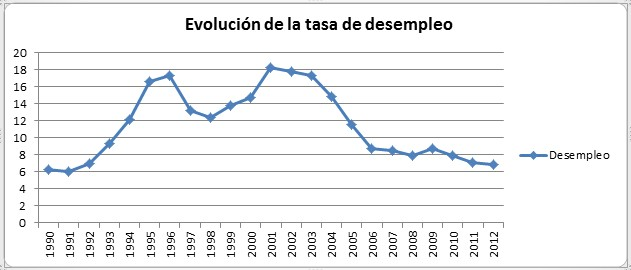
\includegraphics[width=15cm]{images/desocupacion.jpg}
\caption{Gráfico de serie de tiempo de la evolución del desempleo en Argentina \label{desocupacion}}
\end{figure}


\subsection*{¿Para qué queremos series de tiempo?}

Hay varios motivos por los cuales uno querría efectuar un análisis de una serie de tiempo.

\emph{1) Descripción} Usualmente, lo primero que se hace al obtener la serie de tiempo es graficarla y obtener las características más notorias de ésta. Por ejemplo, en \ref{desocupacion} puede notarse que hay una tendencia decreciente del $2003$ hasta el $2012$. En otras (como en el volumen de lluvias) podrá observarse cierta estacionalidad en la serie.

Si bien ésto no requiere técnicas avanzadas de análisis, es el primer paso fundamental para comprender una serie de tiempo.


\emph{2) Explicación} Cuando analizamos dos o más series de tiempo, podemos querer ver cómo se comportan en conjunto. Una variación en una serie de tiempo puede producir un cambio en otra. Por ejemplo, podemos intentar buscar como varían en conjunto la temperatura diaria con la cantidad de mL de lluvia caídos.

\emph{3) Predicción} Dada una serie de tiempo, podemos querer intentar predecir un valor futuro.

\emph{4) Control} Dado un proceso del que se mide cierto parámetro de calidad, podemos querer ajustar variables de entrada para mantenerla en ciertos valores.

En nuestro caso, nos es de interés 1 y 2.


\subsection{Procesos estocásticos}

\begin{definicion}
Una proceso estocástico es una colección de variables aleatorias $\{X_t \}_{t \in T}$ donde $T$ es un conjunto de puntos de tiempo. En nuestro caso, nos interesa $T = \mathbb{N}$, de manera que el proceso será de la forma $X_1, X_2, \ldots $
\end{definicion}

Podemos entender un proceso estocástico como un conjunto de variables ordenadas por el tiempo. Llamamos serie de tiempo a una observación de este proceso estocástico. Usualmente sólo tendremos esta instancia, a diferencia de otros problemas estadísticos donde tendremos muchas observaciones.


\subsection{Estacionariedad}

Un concepto importante en series de tiempo es el de estacionariedad. En lenguaje coloquial, una serie de tiempo estacionaria es aquella en la que no observamos cambios sistemáticos de ésta en el tiempo: si tomamos una parte de la serie, y observamos otro parte distinta de la serie, las propiedades de ésta se mantienen.

Ejemplos de series de tiempo estacionarias son las de ruido blanco, y ejemplos de no estacionarias aquellas que tienen una tendencia. (mejorar esto...)

\begin{definicion}
Un proceso estocástico $X_i, i \in \mathbb{N}$ se dice fuertemente estacionario si, para todo conjunto de índices $t_1, \ldots , t_n$ y para un desplazamiento $\tau \in \mathbb{N}$ tenemos que

\begin{displaymath}
    F_{X_{t_1}, X_{t_2}, \ldots , X_{t_n} } = F_{X_{t_1} + \tau, X_{t_2} + \tau, \ldots , X_{t_n} + \tau}
\end{displaymath}

Es decir, que la función de probabilidad se preserva por traslados.
\end{definicion}

Se derivan como propiedades que, para todo $X_t$ y cualquier desplazamiento $\tau$

\begin{align}
    E[X_t] &= E[X_{t + \tau}] \label{eq:1} \\
    Var[X_t] &= Var[X_{t + \tau}] \label{eq:2} \\
    Cov(X_s, X_t) &= Cov(X_{s+\tau}, X_{t + \tau}) \label{eq:3}
\end{align}

Las ecuaciones \ref{eq:1} y \ref{eq:2} nos dicen que tanto la media como la varianza son constantes (no dependen de $t$), y que la covarianza sólo depende de la diferencia $| s - t |$.


\begin{definicion}
    Un proceso se dice débilmente estacionario si cumple \ref{eq:1}, \ref{eq:2}, \ref{eq:3}
\end{definicion}

A partir de aquí, cuando hablemos de series estacionarias estaremos hablando de series débilmente estacionarias


\section{Descripción TAMA}
\label{sec:ant_tama}

En \cite{KOU2008} se introdujo un método novedoso para el análisis del \entrainment acústico/prosódico. Esta técnica consiste, a grandes rasgos, en armar dos series de tiempo para cada uno de los interlocutores y luego utilizar herramientes de análisis sobre las series construídas. Una serie de tiempo, en términos coloquiales, es una colección cronológica de observaciones, como pueden ser los valores de las acciones de una empresa a lo largo del tiempo, o la cantidad de lluvia medida en \emph{ml} para cada mes de cierto año. En el apéndice \ref{sec:time_series} describimos más en detalle los conceptos básicos sobre series de tiempo.

Un problema que resuelve esta técnica es el del alineamiento: si intentásemos comparar cada segmento del habla (utterance) con otros, ¿cómo los alineamos? Una posibilidad sería uno a uno, aunque ésto es muy simplista y poco representativo de la realidad. Al introducir el concepto de series de tiempo, podemos olvidarnos de los segmentos del habla y simplemente utilizar estas construcciones.

Para construir la serie de tiempo de cada interlocutor debemos, en primer lugar, dividir el diálogo en ventanas solapadas de igual tamaño. A la diferencia entre ventana y ventana llamaremos \emph{frame step}, y al tamaño de ventana \emph{frame length}. Consideraremos sólo los segmentos de habla que se encuentren dentro de cada ventana; aquellos segumentos que atraviesen los límites de las ventanas son cortados para que se mantengan dentro de éste. En la figura \ref{tama} se ilustra el proceso.

Como producto de ésto, nuestro corpus queda dividido en una sucesión ventanas solapadas. En el trabajo original, se usa un step de 10 segundos, y un tamaño de ventana de 20 segundos. Ésto da como resultado un solapamiento del 50\%. En la sección \ref{sec:window_selection}, describimos la elección del tamaño de ventana que hicimos en base al corpus que utilizamos.

\begin{figure}
\centering
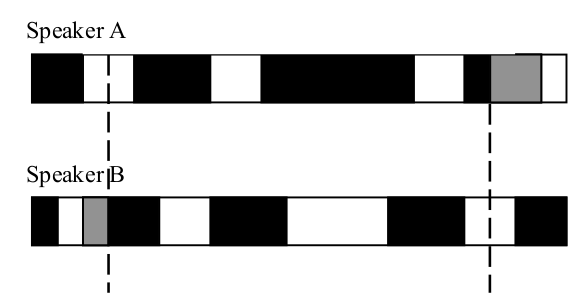
\includegraphics[width=10cm]{images/tama.png}
\caption{Gráfico de la separación del diálogo en ventanas}
\label{tama}
\end{figure}

Una vez que la conversación se ha partido en ventanas mediante el proceso descripto, se calculan los valores de la serie de tiempo para cada interlocutores de cada una de ellas. Ésto se hace mediante el siguiente cálculo:

\begin{equation}
    \mu = \sum\limits_{i=1}^N f_i d_i^\prime \label{eq:tama_mean}\\
\end{equation}

donde $i$ itera sobre las elocuciones dentro del \emph{frame}, $d_i^\prime$ es la duración relativa del segmento (respecto del tiempo total hablado) y $f_i$ es el valor de la \emph{feature} que estamos midiendo. $d_i^\prime$ se calcula con la fórmula

\begin{equation}
dr_i = \frac{d_i}{\sum\limits_{i=1}^N d_i}
\end{equation}

donde $d_i$ es la longitud en segundos de los segmentos del habla en el frame.

Como se ve en \ref{eq:tama_mean}, el valor que calculamos es una media ponderada del valor de la feature por la duración de las locuciones. Así, por ejemplo, al calcular una serie de tiempo sobre la intensidad, la contribución de interjecciones (\emph{ah!} por ejemplo), que suelen tener altos valores \emph{volumen}, estará disminuída por sus breves duraciones.

Una vez obtenidas, dado un feature acústico/prosódico y una conversación, dos series de tiempo mediante el cálculo ventana a ventana de \ref{eq:tama_mean}, necesitamos efectuar algún tipo de análisis sobre éstas para obtener una medida del \entrainment.

\nota{Mejorar el dibujo éste y agregarle una descripción}

\section{Análisis bivariado}
\label{sec:analisis_bivariado}

\newcommand{\squarederr}[1]{
    \sum\limits_{t=1}^n \varnorm{#1}^2
}

\newcommand{\crosscorr}[2]{
  \frac{\sum\limits_{t=|k|+1}^n \varnorm{#1} (#2_{t-k} - \mu_{#2})}{
    \sqrt{\squarederr{#1} \squarederr{#2}}
  } \\
}

\newcommand{\corrdenom}{\sqrt{\squarederr{A}\squarederr{B}}}

En \cite{KOU2008.2} se continúa el trabajo en series de tiempo, y se efectúan análisis tanto para cada serie por separado como para las dos en conjunto, lo cual se llama ``análisis bivariado'' en la terminología de series de tiempo. En este análisis pretendemos analizar ambas series como parte de un sistema y ver cómo se influyen y retroalimentan mutuamente.

Una posible medida del \entrainment se podría obtener midiendo cuánto influye una serie sobre otra, considerándolas a ambas como parte de un sistema donde ambas interactúan. Este \entrainment, entonces, sería direccional: queremos medir cuánto influye el interlocutor $A$ sobre el interlocutor $B$ y viceversa. Puede darse el caso en que ambos tengan fuerte interacción, en tal caso hablamos de \emph{feedback}.

Para medir cuánto se mimetizan las dos series, utilizaremos la función de correlación cruzada (f.c.c) \cite{CHATFIELD}, que mide cuánto se parecen la serie $X$ e $Y$ aplicando un desplazamiento $k$, lo cual nos arroja como resultado un valor entre $-1$ y $1$ (similar al coeficiente de correlación de la estadística clásica). Podemos aproximar la c.c.f. mediante la fórmula de la correlación cruzada muestral.

\begin{equation}
  \label{cross_correlation_definition}
  r_{AB}(k) =
  \left\{
    \begin{array}{ll}
      \frac{\sum\limits_{t=k+1}^n \varnorm{A} (B_{t-k} - \mu_{B})}{\corrdenom} \\ & \mbox{si } k \geq 0 \\
      \frac{\sum\limits_{t=-k+1}^n \varnorm{B} (A_{t+k} - \mu_{A})}{\corrdenom} \\  & \mbox{si } k < 0
    \end{array}
  \right.
\end{equation}

Podemos ver que, si $k \geq 0$, lo que hacemos es, a grandes rasgos, calcular la correlación de Pearson entre $A$ y $B$, pero tomando los $n-k$ últimos valores de $A$ y los $n-k$ primeros de $B$. Si $k < 0$, lo hacemos entre $A$ y $B$, pero desplazando en sentidos inversos. Viéndolo de otra forma, si $k \geq 0$, estamos midiendo cuánto influye $B$ sobre $A$ contemplando un desplazamiento de $k$ puntos; si $k \leq 0$ medimos la influencia de $A$ sobre $B$ a misma distancia. La utilización de estos desplazamientos está explicada en \cite{gravano2015backward}, donde se menciona que la influencia de los hablantes no es necesariamente inmediata sino que puede tener algunos segundos de demora para tomar lugar.


Para cada conversación, se estima entonces el correlograma cruzado, considerando desplazamientos tanto positivos como negativos. Hecho esto, en el estudio \cite{KOU2008.2} sólo analizan la significancia de los resultados de la correlación cruzada, enumerando aquellos lags en los cuales esto ocurrió. En la sección \ref{sec:method_entrainment} comentaremos cómo utilizamos la técnica descripta para la medición del entrainment direccional.

\begin{figure}
\centering
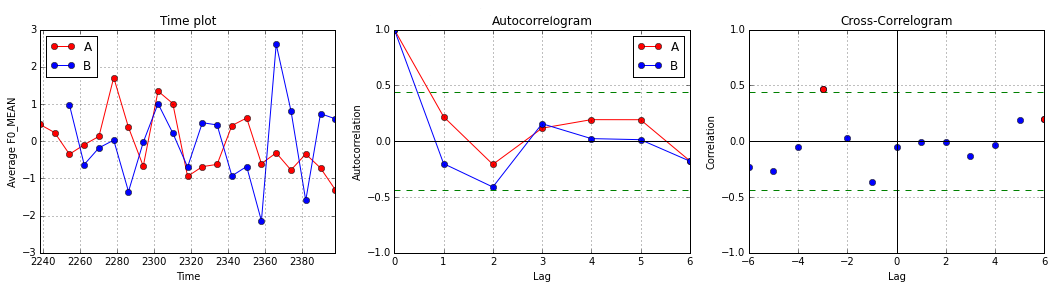
\includegraphics[width=15cm]{images/time_plot_with_cross_correlation.png}
\caption{Time-plot producido por TAMA, junto a su autocorrelación y correlación cruzada}
\end{figure}



\chapter{Corpus}
\section{Columbia Game Corpus}

\newcommand{\objectgame} {\emph{Juego de objetos}}


Empleamos el Columbia Game Corpus  \cite{GRAV2009} consiste en doce conversaciones diádicas (i.e., con dos participantes) entre trece personas angloparlantes distintas. Todos los participantes reportaron hablar Inglés Americano Estándar, y no tener problemas de audición. La edad de los participantes se encuentra en el rango de los 20 a 50 años.

Las grabaciones se hicieron en 44 kHz, 16 bits con un canal separado para cada hablante; luego fueron guardadas en 16 kHz para el presente estudio. Cada sesión duró aproximadamente 45 minutos, totalizando 9 horas de
diálogos, 70.259 palabras (2.037 únicas) para todo el cuerpo de datos.

En cada sesión, se sentó a dos participantes (quienes no se conocían previamente) en una cabina profesional de grabación, cara a cara a ambos lados de una mesa, y con una cortina opaca colgando entre ellos para evitar la comunicación visual. Los participantes contaron con sendas computadoras portátiles conectadas entre sí, en las cuales jugaron una serie de juegos simples que requerían de comunicación verbal. El primero de ellos, un juego de cartas que no consideramos en el presente estudio por tratarse esencialmente de monólogos o diálogos con poca interacción. Luego de esto, pasaron al juego que analizamos, denominado `juego de objetos'.

\subsection{Juego de Objetos}

En el juego de objetos, la pantalla de cada jugador mostró un tablero con varios objetos, entre 5 y 7, como se ve en la figura \ref{objects_game}.
Para uno de los jugadores (el Descriptor) el objeto \emph{Objetivo} aparecía en una posición aleatoria entre otros objetos. Para el otro jugador, a quien llamaremos el Seguidor, el objetivo aparecía en la parte baja de la pantalla. Entonces, al Descriptor se le encargaba describir la posición del Objetivo de manera que el Seguidor pudiera mover su representación del objeto a la misma posición en su pantalla. Luego de una negociación entre ambos jugadores para decidir la mejor posición del objeto, se les asignó a los jugadores una puntuación entre 1 y 100 puntos de acuerdo a qué tan acertado fue el posicionamiento del objetivo por parte del Seguidor.

\begin{figure}
\centering
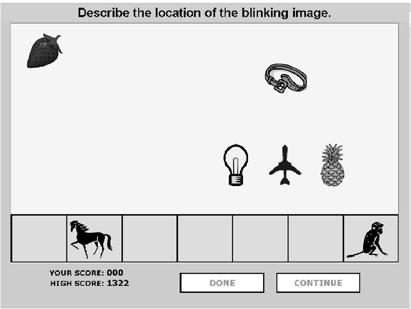
\includegraphics[scale=0.5]{images/columbia_games.jpg}
\caption{Juego de objetos del Columbia Games}
\label{objects_game}
\end{figure}


Cada sesión consistió de 14 tareas como ésta, cambiando los objetos y sus ubicaciones. En las primeras cuatro tareas, uno de los sujetos tomó el papel del Descriptor; en los siguientes cuatro invirtieron roles, y en las finales seis fueron alternando los roles de Descriptor y Seguidor.

\subsection{Anotaciones sobre comportamiento social}

Varios aspectos del comportamiento de los jugadores durante los juegos de objetos fueron anotados mediante la herramienta de crowdsourcing \emph{Amazon Mechanical Turk}. Cada anotador escuchó el audio correspondiente a una tarea del juego y tuvo que responder a varias preguntas sobre cada uno de los sujetos, entre las que se encuentran:

\begin{itemize}
  \item ¿el sujeto parece comprometido con el juego?
  \item ¿el sujeto dirige la conversación?
  \item ¿el sujeto contribuye para el éxito del equipo?
  \item ¿el sujeto alienta a su compañero?
  \item ¿el sujeto se expresa correctamente?
  \item ¿al sujeto no le agrada su compañero?
  \item ¿el sujeto le hace difícil hablar a su compañero?
  \item ¿el sujeto intenta acaparar la conversación?
\end{itemize}

\noindent Cada uno de estos audios fue puntuado por cinco anotadores, que respondieron por sí o por no para cada una de las preguntas. El puntaje que recibe cada una de las preguntas (a las cuales llamaremos a partir de ahora \emph{variables sociales}) consiste en la cantidad de respuestas afirmativas que recibió, teniendo un rango de 0 a 5. Por ejemplo, una tarea dada podría tener puntaje 3 para la variable social `el sujeto A se expresa correctamente' o puntaje 5 para la variable `el sujeto B dirige la conversación'.

\subsection{Extracción de variables acústico/prosódicas}

La herramienta \emph{Praat} fue utilizada para extraer automáticamente las variables \ap del corpus. Las variables que medimos fueron el tono, la intensidad, la proporción de vocalizaciones, jitter, shimmer, cantidad de sílabas, cantidad de fonemas, y la proporción de ruido sobre armónicos. Estos atributos fueron medidos en cada uno de los segmentos de habla del corpus.

Repasemos algunos conceptos que necesitamos para definir las variables acústicas.

\begin{itemize}
  \item \emph{f0} refiere a la frecuencia fundamental de una onda, que es el recíproco del período de ésta. El \emph{tono} o \emph{pitch} es la percepción que tenemos de la frecuencia fundamental, que nos marca cuán agudos o graves son los sonidos.
  \item \emph{Intensity} refiere al volumen o intensidad de la onda. Ésta mide la amplitud de la onda, y es la percepción de cuán fuerte es el sonido.
  \item \emph{jitter y shimmer} se refieren, en un intervalo de tiempo, a los desplazamientos de la onda de la verdadera periodicidad y de la amplitud, respectivamente. Están asociadas con la percepción de la calidad de la voz.
  \item Un \emph{fonema} es la articulación simple de sonidos del habla, tanto de vocales como de consonantes. Ejemplos de fonemas son los sonidos de las letras u, a, s, k en español.
  \item El \emph{noise-to-harmonics ratio} (abreviado NHR) puede considerarse como una medida de calidad de la voz, que cuantifica la proporción de ruido que hay en ésta.
\end{itemize}


En la siguiente tabla resumimos estas features. Recordemos nuevamente que estas features son medidas en un intervalo de tiempo.

\begin{figure}[h!]
\centering
\resizebox{\textwidth}{!}{
\begin{tabular} {|c|c|}
  \hline
  Variable a/p & Descripción \\
  \hline
  \hline
  \FOMEAN & Valor medio de la frecuencia fundamental \\\hline
  \FOMAX  & Valor máximo de la frecuencia fundamental \\\hline
  \ENGMEAN & Valor medio de la intensidad \\\hline
  \ENGMAX & Valor máximo de la intensidad \\\hline
  \NOISETOHARMONICS & Noise-to-harmonics descripto anteriormente \\\hline
  \LOCALSHIMMER & Shimmer medido \\\hline
  \SYLAVG & Cantidad de sílabas por segundo \\\hline
  \PHONAVG & Cantidad de fonemas por segundo \\\hline
\end{tabular}
}
\end{figure}


\chapter{Método}
\section{Selección de Ventana}

En \cite{KOU2009} se menciona una elección de \emph{frame step} y \emph{frame length} de 10s y 20s respectivamente. En el caso de nuestro corpus, quisimos buscar los parámetros que mejor se ajustaban a éste, manteniendo la superposición del 50\% entre ventanas sucesivas. Con lo que nos queda que $FL = 2 * FS$

¿Qué queremos optimizar? La métrica que elegimos para ésto es encontrar un balance entre un frame no tan grande (para no suavizar en exceso la curva) y que nos reduzca considerablemente la cantidad de indefiniciones; es decir, aquellas ventanas que tomamos en un interlocutor que no tienen ninguna interacción de su parte. Para ver ésto, graficamos la cantidad de indefiniciones en función del step tomado.

\begin{figure}
\centering
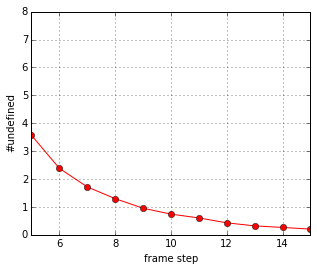
\includegraphics[width=10cm]{images/window_selection.png}
\end{figure}



Dentro del rango de $FS \in \{5'',6'', \ldots ,15'' \}$, graficamos para cada sesión, tarea y cada interlocutor las curvas de indefiniciones. A su vez, para mayor claridad, graficamos una curva que promedie todas las tareas de una sesión.


Para tener una visión general de lo que ocurría en todas las sesiones, graficamos una curva promedio de todas las sesiones. En ésta puede observarse que hasta $8''-10''$ hay un fuerte descenso de las indefiniciones, que luego se atenúa. Dado que en general tenemos tareas cortas, preferimos tomar $8''$ como step, y $16''$ como largo de ventana.

OBS: podríamos cambiar ésto a un boxplot!

\begin{figure}
\centering
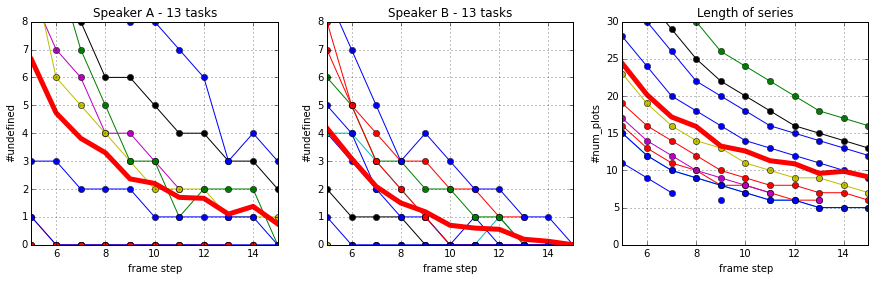
\includegraphics[height=5cm]{images/window_selection_for_session.png}
\end{figure}

\section{Time plots}
\label{sec:time_plots}
Usando la técnica descripta con las variaciones que consideramos en la anterior sección, generamos dos series de tiempo para cada tarea. Como antes mencionamos, la ventana elegida es de 16 segundos con un step de 8 segundos lo cual da un overlap del 50\%.

Dada una ventana, puede ocurrir que alguno de los interlocutores no haya hablado, o su interacción haya sido demasiado breve como para medir sus variables \ap. Como ya mencionamos en la sección \ref{sec:tama_modifications}, y a diferencia de \cite{KOU2008.2}, construimos las series sin ese punto, y sin interpolarlo tampoco.

De estas tareas, sólo nos quedamos con aquellas que tengan al menos 5 puntos definidos para cada serie, de manera que tenga sentido poder calcular la correlación cruzada más adelante. Con esto, no sólo nos interesa la duración de la charla, sino cierta calidad de las series generadas. En la tabla \ref{tab:time_series} pueden verse las tareas que tuvimos en consideración, junto a su duración.

\begin{table}
\centering

\adjustbox{max width=\textwidth}{\begin{tabular}{lllllllllllll}
\toprule
Task & S-01 & S-02 & S-03 & S-04 & S-05 & S-06 & S-07 & S-08 & S-09 & S-10 & S-11 & S-12 \\
\midrule
01 &         -- &         -- &    149.888 &         -- &         -- &         -- &         -- &         -- &     54.514 &    106.096 &         -- &     56.135 \\
02 &         -- &         -- &         -- &         -- &         -- &         -- &         -- &         -- &     41.711 &     63.837 &         -- &         -- \\
03 &         -- &     51.762 &         -- &     80.737 &     77.977 &     69.260 &     68.489 &     49.607 &         -- &    122.272 &     81.037 &         -- \\
04 &         -- &    187.201 &     93.333 &     76.131 &     79.946 &     99.240 &     84.342 &         -- &     58.020 &    129.621 &     67.977 &     95.292 \\
05 &         -- &         -- &         -- &     86.336 &         -- &    126.759 &    145.849 &     90.742 &     45.773 &    134.206 &         -- &         -- \\
06 &         -- &         -- &         -- &         -- &         -- &    148.218 &     50.672 &     60.281 &     46.165 &     66.762 &     46.773 &     40.200 \\
07 &         -- &     66.024 &         -- &    117.762 &         -- &     72.410 &         -- &     87.702 &     85.900 &    110.675 &     65.758 &         -- \\
08 &         -- &    458.885 &     98.681 &    203.867 &         -- &    188.708 &     59.933 &     48.144 &         -- &    157.442 &         -- &     81.165 \\
09 &         -- &         -- &         -- &     75.551 &    134.247 &     83.045 &    108.786 &         -- &     62.128 &    404.014 &     41.097 &     92.555 \\
10 &     50.131 &    231.392 &    162.895 &    242.588 &         -- &    122.408 &     71.198 &     74.775 &         -- &    356.079 &     69.834 &     92.769 \\
11 &         -- &     74.400 &         -- &     98.634 &     70.189 &         -- &     58.911 &         -- &     72.947 &    104.036 &     59.495 &    101.970 \\
12 &     61.331 &     90.100 &    129.129 &    182.917 &         -- &    130.375 &     75.891 &     57.656 &         -- &    101.661 &         -- &     64.842 \\
13 &     55.146 &    124.095 &    108.196 &    144.193 &    114.720 &         -- &         -- &     83.828 &     94.087 &    174.009 &     84.824 &     91.525 \\
14 &         -- &     75.334 &         -- &         -- &    107.356 &         -- &     52.583 &    144.378 &     75.589 &    108.456 &     91.648 &     98.487 \\
\bottomrule
\end{tabular}
}

\caption{Tabla de tareas seleccionadas y sus duraciones}
\label{tab:time_series}
\end{table}


Como primer paso siempre recomendado en el análisis de series de tiempo \cite{CHATFIELD}, graficamos los time plots conjunto de cada par de series, a la vez que sus autocorrelogramas (ver apéndice \ref{sec:time_series}). En la figura \ref{fig:time_plot} podemos observar un ejemplo de esto.

A priori, las series tienen aspecto de series autoregresivas de orden uno. Es decir, series que son de la forma $X_t = \alpha X_{t-1} + e_t + c$, con $e_t$ ruido blanco, $\alpha$ y $c$ constantes. Este hecho es esperable  por la construcción misma del método TAMA, ya que la ventana de cada punto tiene un solapamiento con la ventana anterior. Más aún, uno esperaría que $\alpha \sim 0.5$ ya que nuestras ventanas tienen ese índice de overlap. Los autocorrelogramas de las series, por otro lado, tienen en su mayoría un valor significativo en $k = 1$, el valor del $\alpha$ de la autoregresión.


\begin{figure}
\centering
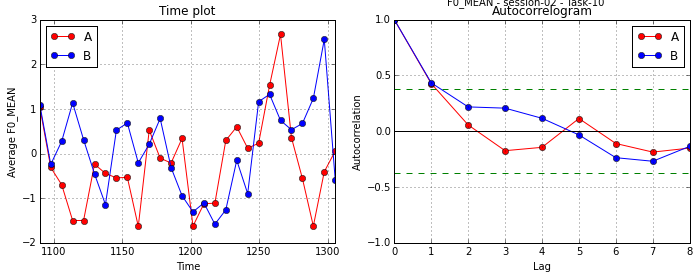
\includegraphics[width=15cm]{images/time_plot_with_autocorrelation.png}
\caption{Time-plot generado por el método TAMA, junto a su autocorrelograma}
\label{fig:time_plot}
\end{figure}

El hecho de que los autocorrelogramas desciendan rápidamente a cero es un indicio de que las series de tiempo construidas son estacionarias, como se menciona en la Sección \ref{sec:autocorrelation}. Esto nos habilita a efectuar el análisis bivariado de las series.

%En esta sección describiremos tanto el corpus utilizado en el estudio, como así también las modificaciones que efectuamos sobre el método TAMA.

\section{Columbia Game Corpus}

\newcommand{\objectgame} {\emph{Juego de objetos}}


Empleamos el Columbia Game Corpus  \cite{GRAV2009} consiste en doce conversaciones diádicas (i.e., con dos participantes) entre trece personas angloparlantes distintas. Todos los participantes reportaron hablar Inglés Americano Estándar, y no tener problemas de audición. La edad de los participantes se encuentra en el rango de los 20 a 50 años.

Las grabaciones se hicieron en 44 kHz, 16 bits con un canal separado para cada hablante; luego fueron guardadas en 16 kHz para el presente estudio. Cada sesión duró aproximadamente 45 minutos, totalizando 9 horas de
diálogos, 70.259 palabras (2.037 únicas) para todo el cuerpo de datos.

En cada sesión, se sentó a dos participantes (quienes no se conocían previamente) en una cabina profesional de grabación, cara a cara a ambos lados de una mesa, y con una cortina opaca colgando entre ellos para evitar la comunicación visual. Los participantes contaron con sendas computadoras portátiles conectadas entre sí, en las cuales jugaron una serie de juegos simples que requerían de comunicación verbal. El primero de ellos, un juego de cartas que no consideramos en el presente estudio por tratarse esencialmente de monólogos o diálogos con poca interacción. Luego de esto, pasaron al juego que analizamos, denominado `juego de objetos'.

\subsection{Juego de Objetos}

En el juego de objetos, la pantalla de cada jugador mostró un tablero con varios objetos, entre 5 y 7, como se ve en la figura \ref{objects_game}.
Para uno de los jugadores (el Descriptor) el objeto \emph{Objetivo} aparecía en una posición aleatoria entre otros objetos. Para el otro jugador, a quien llamaremos el Seguidor, el objetivo aparecía en la parte baja de la pantalla. Entonces, al Descriptor se le encargaba describir la posición del Objetivo de manera que el Seguidor pudiera mover su representación del objeto a la misma posición en su pantalla. Luego de una negociación entre ambos jugadores para decidir la mejor posición del objeto, se les asignó a los jugadores una puntuación entre 1 y 100 puntos de acuerdo a qué tan acertado fue el posicionamiento del objetivo por parte del Seguidor.

\begin{figure}
\centering
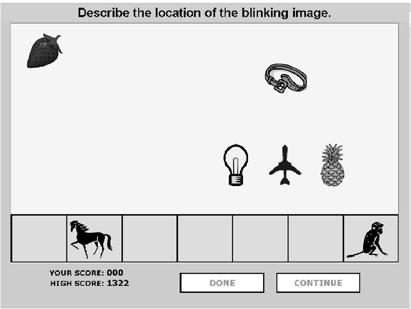
\includegraphics[scale=0.5]{images/columbia_games.jpg}
\caption{Juego de objetos del Columbia Games}
\label{objects_game}
\end{figure}


Cada sesión consistió de 14 tareas como ésta, cambiando los objetos y sus ubicaciones. En las primeras cuatro tareas, uno de los sujetos tomó el papel del Descriptor; en los siguientes cuatro invirtieron roles, y en las finales seis fueron alternando los roles de Descriptor y Seguidor.

\subsection{Anotaciones sobre comportamiento social}

Varios aspectos del comportamiento de los jugadores durante los juegos de objetos fueron anotados mediante la herramienta de crowdsourcing \emph{Amazon Mechanical Turk}. Cada anotador escuchó el audio correspondiente a una tarea del juego y tuvo que responder a varias preguntas sobre cada uno de los sujetos, entre las que se encuentran:

\begin{itemize}
  \item ¿el sujeto parece comprometido con el juego?
  \item ¿el sujeto dirige la conversación?
  \item ¿el sujeto contribuye para el éxito del equipo?
  \item ¿el sujeto alienta a su compañero?
  \item ¿el sujeto se expresa correctamente?
  \item ¿al sujeto no le agrada su compañero?
  \item ¿el sujeto le hace difícil hablar a su compañero?
  \item ¿el sujeto intenta acaparar la conversación?
\end{itemize}

\noindent Cada uno de estos audios fue puntuado por cinco anotadores, que respondieron por sí o por no para cada una de las preguntas. El puntaje que recibe cada una de las preguntas (a las cuales llamaremos a partir de ahora \emph{variables sociales}) consiste en la cantidad de respuestas afirmativas que recibió, teniendo un rango de 0 a 5. Por ejemplo, una tarea dada podría tener puntaje 3 para la variable social `el sujeto A se expresa correctamente' o puntaje 5 para la variable `el sujeto B dirige la conversación'.

\subsection{Extracción de variables acústico/prosódicas}

La herramienta \emph{Praat} fue utilizada para extraer automáticamente las variables \ap del corpus. Las variables que medimos fueron el tono, la intensidad, la proporción de vocalizaciones, jitter, shimmer, cantidad de sílabas, cantidad de fonemas, y la proporción de ruido sobre armónicos. Estos atributos fueron medidos en cada uno de los segmentos de habla del corpus.

Repasemos algunos conceptos que necesitamos para definir las variables acústicas.

\begin{itemize}
  \item \emph{f0} refiere a la frecuencia fundamental de una onda, que es el recíproco del período de ésta. El \emph{tono} o \emph{pitch} es la percepción que tenemos de la frecuencia fundamental, que nos marca cuán agudos o graves son los sonidos.
  \item \emph{Intensity} refiere al volumen o intensidad de la onda. Ésta mide la amplitud de la onda, y es la percepción de cuán fuerte es el sonido.
  \item \emph{jitter y shimmer} se refieren, en un intervalo de tiempo, a los desplazamientos de la onda de la verdadera periodicidad y de la amplitud, respectivamente. Están asociadas con la percepción de la calidad de la voz.
  \item Un \emph{fonema} es la articulación simple de sonidos del habla, tanto de vocales como de consonantes. Ejemplos de fonemas son los sonidos de las letras u, a, s, k en español.
  \item El \emph{noise-to-harmonics ratio} (abreviado NHR) puede considerarse como una medida de calidad de la voz, que cuantifica la proporción de ruido que hay en ésta.
\end{itemize}


En la siguiente tabla resumimos estas features. Recordemos nuevamente que estas features son medidas en un intervalo de tiempo.

\begin{figure}[h!]
\centering
\resizebox{\textwidth}{!}{
\begin{tabular} {|c|c|}
  \hline
  Variable a/p & Descripción \\
  \hline
  \hline
  \FOMEAN & Valor medio de la frecuencia fundamental \\\hline
  \FOMAX  & Valor máximo de la frecuencia fundamental \\\hline
  \ENGMEAN & Valor medio de la intensidad \\\hline
  \ENGMAX & Valor máximo de la intensidad \\\hline
  \NOISETOHARMONICS & Noise-to-harmonics descripto anteriormente \\\hline
  \LOCALSHIMMER & Shimmer medido \\\hline
  \SYLAVG & Cantidad de sílabas por segundo \\\hline
  \PHONAVG & Cantidad de fonemas por segundo \\\hline
\end{tabular}
}
\end{figure}

\section{Modificaciones a TAMA}
\label{sec:tama_modifications}
Al método TAMA descripto en \ref{sec:ant_tama} le hemos aplicado algunas variaciones, que pasaremos a detallar.

En primer lugar, \cite{KOU2008.2} discute la disyuntiva de elegir un tamaño de ventana y step para el método: ventanas demasiado chicas pueden causar que no hayan segmentos de habla en ellas, mientras que un tamaño de ventana demasiado grande suavizaría en exceso la serie de tiempo. A colación de esto, dicho trabajo menciona dos posibles soluciones para el problema de los puntos faltantes: interpolar (también mencionado en \cite{DEL2013}) o repetir el punto anterior de la serie.

Estos enfoques, sin embargo, pueden dar lugar a valores de \entrainment artificialmente altos por la construcción misma de la serie, ya que nos generaría puntos correlacionados fuertemente entre sí en cada una de las series de los hablantes. Por otro lado, descartar aquellas conversaciones que tengan puntos faltantes puede ser demasiado restrictivo y eliminar de nuestro corpus una gran cantidad de datos valiosos. Teniendo estas cosas en mente, decidimos aceptar series de tiempo con datos faltantes, que pueden ser producto de ventanas sin segmentos de habla o con algunos demasiado pequeños que imposibiliten la medición de las variables \ap: por ejemplo interjecciones o backchanneling (\emph{uh-huh} o \emph{hmmm} en inglés).

\section{Selección de Ventana}

En \cite{KOU2009} se menciona una elección de \emph{frame step} y \emph{frame length} de 10s y 20s respectivamente. En el caso de nuestro corpus, quisimos buscar los parámetros que mejor se ajustaban a éste, manteniendo la superposición del 50\% entre ventanas sucesivas. Con lo que nos queda que $FL = 2 * FS$

¿Qué queremos optimizar? La métrica que elegimos para ésto es encontrar un balance entre un frame no tan grande (para no suavizar en exceso la curva) y que nos reduzca considerablemente la cantidad de indefiniciones; es decir, aquellas ventanas que tomamos en un interlocutor que no tienen ninguna interacción de su parte. Para ver ésto, graficamos la cantidad de indefiniciones en función del step tomado.

\begin{figure}
\centering
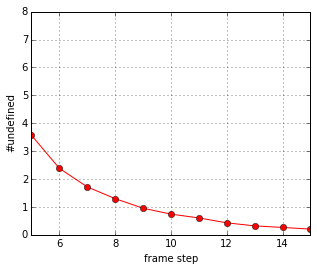
\includegraphics[width=10cm]{images/window_selection.png}
\end{figure}



Dentro del rango de $FS \in \{5'',6'', \ldots ,15'' \}$, graficamos para cada sesión, tarea y cada interlocutor las curvas de indefiniciones. A su vez, para mayor claridad, graficamos una curva que promedie todas las tareas de una sesión.


Para tener una visión general de lo que ocurría en todas las sesiones, graficamos una curva promedio de todas las sesiones. En ésta puede observarse que hasta $8''-10''$ hay un fuerte descenso de las indefiniciones, que luego se atenúa. Dado que en general tenemos tareas cortas, preferimos tomar $8''$ como step, y $16''$ como largo de ventana.

OBS: podríamos cambiar ésto a un boxplot!

\begin{figure}
\centering
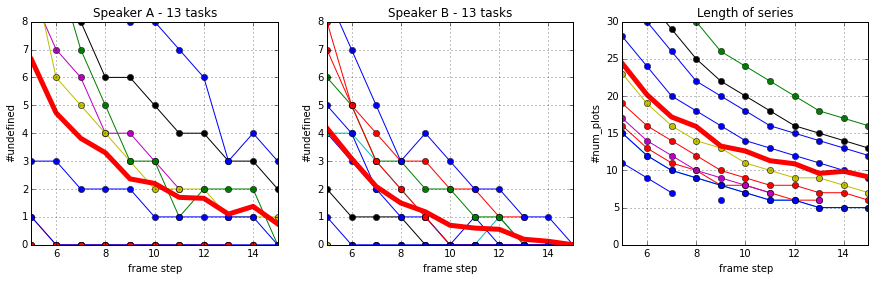
\includegraphics[height=5cm]{images/window_selection_for_session.png}
\end{figure}


\section{Time plots}
\label{sec:time_plots}
Usando la técnica descripta con las variaciones que consideramos en la anterior sección, generamos dos series de tiempo para cada tarea. Como antes mencionamos, la ventana elegida es de 16 segundos con un step de 8 segundos lo cual da un overlap del 50\%.

Dada una ventana, puede ocurrir que alguno de los interlocutores no haya hablado, o su interacción haya sido demasiado breve como para medir sus variables \ap. Como ya mencionamos en la sección \ref{sec:tama_modifications}, y a diferencia de \cite{KOU2008.2}, construimos las series sin ese punto, y sin interpolarlo tampoco.

De estas tareas, sólo nos quedamos con aquellas que tengan al menos 5 puntos definidos para cada serie, de manera que tenga sentido poder calcular la correlación cruzada más adelante. Con esto, no sólo nos interesa la duración de la charla, sino cierta calidad de las series generadas. En la tabla \ref{tab:time_series} pueden verse las tareas que tuvimos en consideración, junto a su duración.

\begin{table}
\centering

\adjustbox{max width=\textwidth}{\begin{tabular}{lllllllllllll}
\toprule
Task & S-01 & S-02 & S-03 & S-04 & S-05 & S-06 & S-07 & S-08 & S-09 & S-10 & S-11 & S-12 \\
\midrule
01 &         -- &         -- &    149.888 &         -- &         -- &         -- &         -- &         -- &     54.514 &    106.096 &         -- &     56.135 \\
02 &         -- &         -- &         -- &         -- &         -- &         -- &         -- &         -- &     41.711 &     63.837 &         -- &         -- \\
03 &         -- &     51.762 &         -- &     80.737 &     77.977 &     69.260 &     68.489 &     49.607 &         -- &    122.272 &     81.037 &         -- \\
04 &         -- &    187.201 &     93.333 &     76.131 &     79.946 &     99.240 &     84.342 &         -- &     58.020 &    129.621 &     67.977 &     95.292 \\
05 &         -- &         -- &         -- &     86.336 &         -- &    126.759 &    145.849 &     90.742 &     45.773 &    134.206 &         -- &         -- \\
06 &         -- &         -- &         -- &         -- &         -- &    148.218 &     50.672 &     60.281 &     46.165 &     66.762 &     46.773 &     40.200 \\
07 &         -- &     66.024 &         -- &    117.762 &         -- &     72.410 &         -- &     87.702 &     85.900 &    110.675 &     65.758 &         -- \\
08 &         -- &    458.885 &     98.681 &    203.867 &         -- &    188.708 &     59.933 &     48.144 &         -- &    157.442 &         -- &     81.165 \\
09 &         -- &         -- &         -- &     75.551 &    134.247 &     83.045 &    108.786 &         -- &     62.128 &    404.014 &     41.097 &     92.555 \\
10 &     50.131 &    231.392 &    162.895 &    242.588 &         -- &    122.408 &     71.198 &     74.775 &         -- &    356.079 &     69.834 &     92.769 \\
11 &         -- &     74.400 &         -- &     98.634 &     70.189 &         -- &     58.911 &         -- &     72.947 &    104.036 &     59.495 &    101.970 \\
12 &     61.331 &     90.100 &    129.129 &    182.917 &         -- &    130.375 &     75.891 &     57.656 &         -- &    101.661 &         -- &     64.842 \\
13 &     55.146 &    124.095 &    108.196 &    144.193 &    114.720 &         -- &         -- &     83.828 &     94.087 &    174.009 &     84.824 &     91.525 \\
14 &         -- &     75.334 &         -- &         -- &    107.356 &         -- &     52.583 &    144.378 &     75.589 &    108.456 &     91.648 &     98.487 \\
\bottomrule
\end{tabular}
}

\caption{Tabla de tareas seleccionadas y sus duraciones}
\label{tab:time_series}
\end{table}


Como primer paso siempre recomendado en el análisis de series de tiempo \cite{CHATFIELD}, graficamos los time plots conjunto de cada par de series, a la vez que sus autocorrelogramas (ver apéndice \ref{sec:time_series}). En la figura \ref{fig:time_plot} podemos observar un ejemplo de esto.

A priori, las series tienen aspecto de series autoregresivas de orden uno. Es decir, series que son de la forma $X_t = \alpha X_{t-1} + e_t + c$, con $e_t$ ruido blanco, $\alpha$ y $c$ constantes. Este hecho es esperable  por la construcción misma del método TAMA, ya que la ventana de cada punto tiene un solapamiento con la ventana anterior. Más aún, uno esperaría que $\alpha \sim 0.5$ ya que nuestras ventanas tienen ese índice de overlap. Los autocorrelogramas de las series, por otro lado, tienen en su mayoría un valor significativo en $k = 1$, el valor del $\alpha$ de la autoregresión.


\begin{figure}
\centering
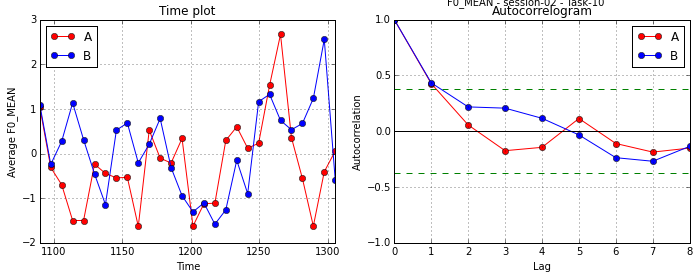
\includegraphics[width=15cm]{images/time_plot_with_autocorrelation.png}
\caption{Time-plot generado por el método TAMA, junto a su autocorrelograma}
\label{fig:time_plot}
\end{figure}

El hecho de que los autocorrelogramas desciendan rápidamente a cero es un indicio de que las series de tiempo construidas son estacionarias, como se menciona en la Sección \ref{sec:autocorrelation}. Esto nos habilita a efectuar el análisis bivariado de las series.

\section{Medición del Entrainment}
\label{sec:method_entrainment}

Considerando todo lo mencionado, procedimos a definir una medida de \entrainment basándonos en el cálculo de la correlación cruzada muestral. Recordemos que, bajo la definición dada en la ecuación \ref{cross_correlation_definition} de $r_{AB}(k)$, al tomar $k \geq 0$ medíamos cuánto influía $B$ sobre los futuros valores de $A$, y viceversa cuando $k \leq 0$. Se tomó la decisión de que este cálculo sólo se realice cuando el desplazamiento resulta en al menos 4 puntos que se solapan; si esto no ocurre, dejamos indefinido el valor en el correlograma cruzado.

Con esto en mente, definimos una primer métrica $\fwentrainment{AB}^{(1)}$ como el valor de $r_{AB}(k)$ con mayor valor absoluto, dado $k \leq 0$. Análogamente lo definimos para $\fwentrainment{BA}^{(1)}$.

En segundo lugar, definimos una segunda métrica $\fwentrainment{BA}^{(2)}$, como el valor absoluto de la primera, es decir:

\begin{equation}
\fwentrainment{BA}^{(2)} = |\fwentrainment{BA}^{(1)}|
\end{equation}

Por último, cabe mencionar que a diferencia de \cite{KOU2008.2} dónde sólo se hacía un análisis de significancia, nosotros vamos a utilizar esta medida independientemente de si es o no estadísticamente diferente de cero.

\section{Panel de datos}
\label{sec:panel_data}

Luego de construir las series de tiempo para cada una de las conversaciones que seleccionamos anteriormente, pasamos a construir una gran tabla que se utilizó en los experimentos de regresión detallados en la siguiente sección. Para condensar todos nuestros datos, armamos una tabla por cada variable acústico-prosódicas, que contiene información definida para cada interlocutor y tarea de nuestro corpus.

Cada columna de esta tabla representa los datos de un interlocutor dentro de una tarea. Éste hecho lo usamos fuertemente a la hora de definir los grupos en nuestro modelo de Efectos Fijos. En la figura \ref{fig:panel_data} se describen las columnas generadas.

\begin{figure}[b!]
\centering
\adjustbox{max width=\textwidth}{
\begin{tabular}{|c|c|}
  \hline
  \myhighlight \emph{Campo} & \emph{Descripción} \\\hline
  session & número de sesión \\\hline
  speaker & 0 si corresponde al interlocutor A; B en otro caso \\\hline
  task & número de tarea \\\hline
  count & La cantidad de puntos definidos que tiene la serie \\\hline
  entrainment & Si $speaker=0$, es $\fwentrainment{AB}$; $\fwentrainment{BA}$ en otro caso \\\hline
  best\_lag & el lag del cross-correlogram donde se logra el \emph{entrainment} \\\hline

  engaged\_in\_game & ¿el sujeto parece comprometido con el juego? \\\hline
  difficult\_for\_partner\_to\_speak & ¿el sujeto dirige la conversación? \\\hline
  contributes\_to\_successful\_completion & ¿el sujeto contribuye para el éxito del equipo? \\\hline
  gives\_encouragement & ¿el sujeto alienta a su compañero?\\\hline
  making\_self\_clear & ¿el sujeto se expresa correctamente?\\\hline

  planning\_what\_to\_say & \\\hline
  bored\_with\_game & ¿el sujeto se muestra aburrido? \\\hline
  dislikes\_partner &  ¿al sujeto no le agrada su compañero? \\\hline
\end{tabular}}
\label{fig:panel_data}
\caption{Columnas de la tabla generada para ser utilizada en los experimentos de regresión lineal}
\end{figure}



La tabla generada tuvo una dimensión de 210 x 21, siendo 210 la cantidad de tareas (contadas dos veces por cada hablante) y 21 las columnas mencionadas en la figura \ref{fig:panel_data}. Una forma de ver ésta tabla es que, para cada sesión y hablante, tenemos una serie de tiempo sobre las tareas   siendo los datos el entrainment y las variables sociales. En la jerga econométrica, llamamos a este tipo de datos \emph{de panel}\cite{gujarati1999}: un conjunto de mediciones temporales sobre un mismo sujeto a lo largo del tiempo. En este caso el sujeto es un interlocutor en una sesión, el tiempo son las tareas, y las mediciones son los entrainments y las diferentes variables sociales.

En la figura \ref{fig:panel_data_example} tenemos una sección de la tabla. Los sujetos que tenemos en éste ejemplo son 3: $speaker = 0$ y $session=1$, $speaker = 1$ y $session=1$, y $speaker = 0$ y $session=2$. También tenemos cinco series de tiempo para cada sujeto: \entrainment, \emph{bored}, \emph{engaged}, \emph{encourages} y \emph{clear}. Vale la pena remarcar que estas series de tiempo, al igual que las que consideramos en la construcción de TAMA, pueden tener datos faltantes.


\begin{figure}
\centering
\adjustbox{max width=\textwidth}{
\begin{tabular}{lrrrrrrrrr}
\toprule
session &  speaker &  task &  entrainment &  bored\_with\_game &  engaged\_in\_game &  gives\_encouragement &  making\_self\_clear &  planning\_what\_to\_say \\
\midrule
1 &        0 &    10 &     0.581475 &                0 &                5 &                    5 &                  5\\
1 &        0 &    12 &    -0.569677 &                1 &                5 &                    5 &                  5\\
1 &        0 &    13 &     0.533701 &                2 &                4 &                    5 &                  4\\
1 &        1 &    10 &    -0.917101 &                0 &                5 &                    2 &                  3\\
1 &        1 &    12 &     0.467112 &                0 &                5 &                    4 &                  2\\
1 &        1 &    13 &    -0.602364 &                0 &                5 &                    4 &                  3\\
2 &        0 &     3 &     0.520696 &                0 &                4 &                    5 &                  5\\
2 &        0 &     4 &    -0.241060 &                0 &                5 &                    4 &                  4\\
2 &        0 &     7 &     0.743719 &                0 &                5 &                    4 &                  5\\
2 &        0 &     8 &     0.147362 &                0 &                5 &                    4 &                  2\\
\bottomrule
\end{tabular}
}


\caption{Ejemplo de tabla generada para $\FOMEAN$}
\label{fig:panel_data_example}
\end{figure}


\begin{figure}
\centering
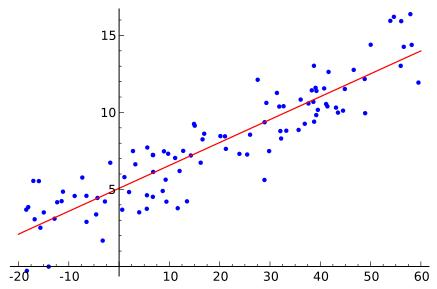
\includegraphics[width=10cm]{images/linear_regression.jpg}
\caption{Ejemplo de Regresión Lineal}
\end{figure}

\section{Análisis de regresión}

Llegado a este punto, dada una variable a/p, nos interesaría evaluar la relación entre el entrainment y las distintas variables sociales. Con esto en mente, planteamos un modelo de regresión lineal donde nuestra variable explicativa será la mimetización, y la variable \emph{dependiente} será la variable social.

En base a ésto, podremos observar cuál es la variación conjunta de ellas. Es esperable que, al aumentar la mimetización, aumenten ciertas variables sociales (por ejemplo, la compenetración en el juego) y que otras desciendan (el aburrimiento).


\subsection{Modelo clásico de Regresión Lineal}

En el modelo clásico de regresión lineal, tenemos un conjunto de valores fijos $X_1, X_2, \ldots, X_n$, que son llamadas variables independientes. Asociado a cada uno de estos valores fijos, tenemos variables aleatorias $Y_1, \ldots, Y_n$. Asumimos, además, que nuestras variables son de la forma

\begin{equation}
  Y_i = E[Y|X_i] + u_i
\end{equation}

donde $u_i$ es la perturbación estocástica de la variable.

Asumiendo que $E[Y|X_i]$ es una función lineal de $X_i$; es decir, que existen $\beta_1, \beta_2 \in \mathbb{R}$ que cumplen

\begin{equation}
  E[Y|X_i] = \beta_1 + \beta_2 X_i
\end{equation}

obtenemos que

\begin{equation}
  Y_i = \beta_1 + \beta_2 X_i + u_i
\end{equation}

Nuestro objetivo es poder entonces conseguir estimadores $\widehat{\beta_1}, \widehat{\beta_2}$ que nos permitan analizar y predecir el comportamiento conjunto de estas variables.

\subsection{Nuestro modelo}

Sea entonces una variable acústica/prosódica (por ejemplo, el pitch o la intensidad), y una variable social de las que acabamos de enumerar en \ref{sec:panel_data}. Sean $E_1, \ldots, E_n$ los valores de entrainment para el set de datos que definimos en \ref{sec:panel_data}, y sean $V_1, V_2, \ldots V_n$ los valores de la variable social de cada conversación.

Sobre éstas variables es que planteamos nuestro modelo de regresión lineal clásica: queremos ver qué relación hay tomando como variable ``fija'' al entrainment, y como variable dependiente a la variable social. Queremos hallar, entonces $\widehat{\beta_1}, \widehat{\beta_2} \in \mathbb{R}$

\begin{equation}
  V_i \simeq \widehat{\beta_1} + \widehat{\beta_2} E_i
\end{equation}


Para ello, calcularemos los estimadores $\widehat{\beta_1}, \widehat{\beta_2} \in \mathbb{R}$ mediante el método \emph{QR} (insertar referencia aquí) que nos provee el lenguaje R. A su vez, luego de ésto efectuaremos un análisis de significancia sobre $\beta_2$ para verificar que sean distintos de 0.


Uno esperaría que un alto \emph{entrainment} se relacione con un alto valor de ciertas variables sociales \cite{BRE1996}, por ejemplo la compenetración con el juego, el ayudar a terminarlo. Esto significa esperar que el valor de $\widehat{\beta_2}$; y se relacione con bajos valores de otras, como el aburrimiento, o el rechazo percibido hacia el compañero.






\section{Panel de datos}
\label{sec:panel_data}

Luego de construir las series de tiempo para cada una de las conversaciones que seleccionamos anteriormente, pasamos a construir una gran tabla que se utilizó en los experimentos de regresión detallados en la siguiente sección. Para condensar todos nuestros datos, armamos una tabla por cada variable acústico-prosódicas, que contiene información definida para cada interlocutor y tarea de nuestro corpus.

Cada columna de esta tabla representa los datos de un interlocutor dentro de una tarea. Éste hecho lo usamos fuertemente a la hora de definir los grupos en nuestro modelo de Efectos Fijos. En la figura \ref{fig:panel_data} se describen las columnas generadas.

\begin{figure}[b!]
\centering
\adjustbox{max width=\textwidth}{
\begin{tabular}{|c|c|}
  \hline
  \myhighlight \emph{Campo} & \emph{Descripción} \\\hline
  session & número de sesión \\\hline
  speaker & 0 si corresponde al interlocutor A; B en otro caso \\\hline
  task & número de tarea \\\hline
  count & La cantidad de puntos definidos que tiene la serie \\\hline
  entrainment & Si $speaker=0$, es $\fwentrainment{AB}$; $\fwentrainment{BA}$ en otro caso \\\hline
  best\_lag & el lag del cross-correlogram donde se logra el \emph{entrainment} \\\hline

  engaged\_in\_game & ¿el sujeto parece comprometido con el juego? \\\hline
  difficult\_for\_partner\_to\_speak & ¿el sujeto dirige la conversación? \\\hline
  contributes\_to\_successful\_completion & ¿el sujeto contribuye para el éxito del equipo? \\\hline
  gives\_encouragement & ¿el sujeto alienta a su compañero?\\\hline
  making\_self\_clear & ¿el sujeto se expresa correctamente?\\\hline

  planning\_what\_to\_say & \\\hline
  bored\_with\_game & ¿el sujeto se muestra aburrido? \\\hline
  dislikes\_partner &  ¿al sujeto no le agrada su compañero? \\\hline
\end{tabular}}
\label{fig:panel_data}
\caption{Columnas de la tabla generada para ser utilizada en los experimentos de regresión lineal}
\end{figure}



La tabla generada tuvo una dimensión de 210 x 21, siendo 210 la cantidad de tareas (contadas dos veces por cada hablante) y 21 las columnas mencionadas en la figura \ref{fig:panel_data}. Una forma de ver ésta tabla es que, para cada sesión y hablante, tenemos una serie de tiempo sobre las tareas   siendo los datos el entrainment y las variables sociales. En la jerga econométrica, llamamos a este tipo de datos \emph{de panel}\cite{gujarati1999}: un conjunto de mediciones temporales sobre un mismo sujeto a lo largo del tiempo. En este caso el sujeto es un interlocutor en una sesión, el tiempo son las tareas, y las mediciones son los entrainments y las diferentes variables sociales.

En la figura \ref{fig:panel_data_example} tenemos una sección de la tabla. Los sujetos que tenemos en éste ejemplo son 3: $speaker = 0$ y $session=1$, $speaker = 1$ y $session=1$, y $speaker = 0$ y $session=2$. También tenemos cinco series de tiempo para cada sujeto: \entrainment, \emph{bored}, \emph{engaged}, \emph{encourages} y \emph{clear}. Vale la pena remarcar que estas series de tiempo, al igual que las que consideramos en la construcción de TAMA, pueden tener datos faltantes.


\begin{figure}
\centering
\adjustbox{max width=\textwidth}{
\begin{tabular}{lrrrrrrrrr}
\toprule
session &  speaker &  task &  entrainment &  bored\_with\_game &  engaged\_in\_game &  gives\_encouragement &  making\_self\_clear &  planning\_what\_to\_say \\
\midrule
1 &        0 &    10 &     0.581475 &                0 &                5 &                    5 &                  5\\
1 &        0 &    12 &    -0.569677 &                1 &                5 &                    5 &                  5\\
1 &        0 &    13 &     0.533701 &                2 &                4 &                    5 &                  4\\
1 &        1 &    10 &    -0.917101 &                0 &                5 &                    2 &                  3\\
1 &        1 &    12 &     0.467112 &                0 &                5 &                    4 &                  2\\
1 &        1 &    13 &    -0.602364 &                0 &                5 &                    4 &                  3\\
2 &        0 &     3 &     0.520696 &                0 &                4 &                    5 &                  5\\
2 &        0 &     4 &    -0.241060 &                0 &                5 &                    4 &                  4\\
2 &        0 &     7 &     0.743719 &                0 &                5 &                    4 &                  5\\
2 &        0 &     8 &     0.147362 &                0 &                5 &                    4 &                  2\\
\bottomrule
\end{tabular}
}


\caption{Ejemplo de tabla generada para $\FOMEAN$}
\label{fig:panel_data_example}
\end{figure}


\begin{figure}
\centering
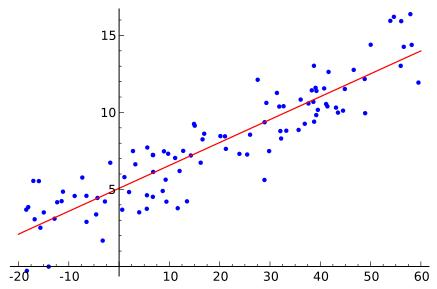
\includegraphics[width=10cm]{images/linear_regression.jpg}
\caption{Ejemplo de Regresión Lineal}
\end{figure}

\section{Análisis de regresión}

Llegado a este punto, dada una variable a/p, nos interesaría evaluar la relación entre el entrainment y las distintas variables sociales. Con esto en mente, planteamos un modelo de regresión lineal donde nuestra variable explicativa será la mimetización, y la variable \emph{dependiente} será la variable social.

En base a ésto, podremos observar cuál es la variación conjunta de ellas. Es esperable que, al aumentar la mimetización, aumenten ciertas variables sociales (por ejemplo, la compenetración en el juego) y que otras desciendan (el aburrimiento).


\subsection{Modelo clásico de Regresión Lineal}

En el modelo clásico de regresión lineal, tenemos un conjunto de valores fijos $X_1, X_2, \ldots, X_n$, que son llamadas variables independientes. Asociado a cada uno de estos valores fijos, tenemos variables aleatorias $Y_1, \ldots, Y_n$. Asumimos, además, que nuestras variables son de la forma

\begin{equation}
  Y_i = E[Y|X_i] + u_i
\end{equation}

donde $u_i$ es la perturbación estocástica de la variable.

Asumiendo que $E[Y|X_i]$ es una función lineal de $X_i$; es decir, que existen $\beta_1, \beta_2 \in \mathbb{R}$ que cumplen

\begin{equation}
  E[Y|X_i] = \beta_1 + \beta_2 X_i
\end{equation}

obtenemos que

\begin{equation}
  Y_i = \beta_1 + \beta_2 X_i + u_i
\end{equation}

Nuestro objetivo es poder entonces conseguir estimadores $\widehat{\beta_1}, \widehat{\beta_2}$ que nos permitan analizar y predecir el comportamiento conjunto de estas variables.

\subsection{Nuestro modelo}

Sea entonces una variable acústica/prosódica (por ejemplo, el pitch o la intensidad), y una variable social de las que acabamos de enumerar en \ref{sec:panel_data}. Sean $E_1, \ldots, E_n$ los valores de entrainment para el set de datos que definimos en \ref{sec:panel_data}, y sean $V_1, V_2, \ldots V_n$ los valores de la variable social de cada conversación.

Sobre éstas variables es que planteamos nuestro modelo de regresión lineal clásica: queremos ver qué relación hay tomando como variable ``fija'' al entrainment, y como variable dependiente a la variable social. Queremos hallar, entonces $\widehat{\beta_1}, \widehat{\beta_2} \in \mathbb{R}$

\begin{equation}
  V_i \simeq \widehat{\beta_1} + \widehat{\beta_2} E_i
\end{equation}


Para ello, calcularemos los estimadores $\widehat{\beta_1}, \widehat{\beta_2} \in \mathbb{R}$ mediante el método \emph{QR} (insertar referencia aquí) que nos provee el lenguaje R. A su vez, luego de ésto efectuaremos un análisis de significancia sobre $\beta_2$ para verificar que sean distintos de 0.


Uno esperaría que un alto \emph{entrainment} se relacione con un alto valor de ciertas variables sociales \cite{BRE1996}, por ejemplo la compenetración con el juego, el ayudar a terminarlo. Esto significa esperar que el valor de $\widehat{\beta_2}$; y se relacione con bajos valores de otras, como el aburrimiento, o el rechazo percibido hacia el compañero.






\chapter{Regresión Lineal Agrupada}
En esta sección, mostraremos el primer experimento que hicimos. Éste consistió en aplicar un modelo de regresión lineal de cada variable social sobre el \entrainment.

Una variación que usaremos en el presente experimento (y en el posterior) es utilizar como variable dependiente el valor absoluto del \entrainment, en base a estudios que sugieren que los interlocutores pueden también diferenciarse como un rasgo positivo en la conversación.

\section{Modelo agrupado o \emph{pooled}}

En el modelo agrupado o \emph{pooled}, no distinguimos entre datos provenientes de distintos ``grupos'' \cite{gujarati1999} y sobre estos calculamos la regresión lineal, agrupando todos los datos disponibles.

Un problema que surge con este tipo de regresión es que niega todo tipo de \emph{heterogeneidad} de los datos: estos pueden provenir de interlocutores más o menos empáticos, o cuya interacción en el juego se vio influída por factores no medidos en el experimento. Todo esto es descartado, aún cuando puede afectar seriamente  el resultado obtenido.

\nota{Gráfico de ejemplo de pooled ols}

\begin{figure}[b!]
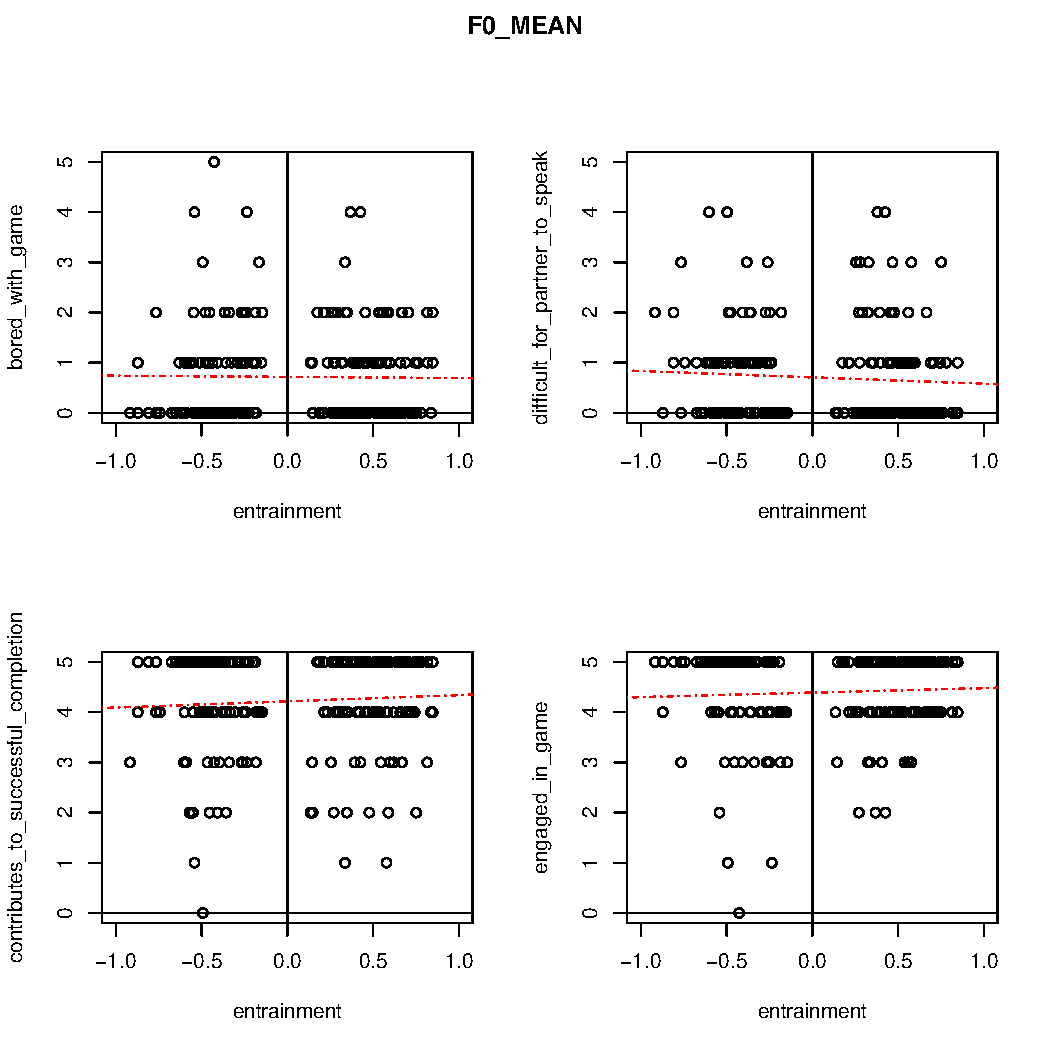
\includegraphics[width=15cm]{images/regression_F0_MEAN_1.pdf}
\caption{Gráfico de los pares entrainment-variable a/p, junto a la regresión lineal obtenida \label{regresion_clasica} para \emph{F0\_MEAN}}
\end{figure}

\section{Resultados sobre \entrainment}

Este modelo dio resultados con baja significancia. En \ref{regresion_clasica} puede verse el gráfico de \emph{F0\_MEAN} y 4 variables sociales y en \ref{regresion_clasica_tabla} pueden verse los valores de las estimaciones de $\estslope$ junto a sus p-valores.

% "ENG_MEAN"
% latex table generated in R 3.2.2 by xtable 1.8-0 package
% Thu Jan  7 03:01:56 2016
\begin{tabular}{rrrrr}
  \hline
 ENG\_MEAN & $\widehat{\beta_2}$ & Std. Error & t value & Pr($>$$|$t$|$) \\
  \hline
  bored\_with\_game & 10.6496 & -0 & 2.036037E-21 & 0.6587 \\
  difficult\_for\_partner\_to\_speak & 10.5625 & -1 & 3.728189E-21 & 0.5893 \\
  contributes\_to\_successful\_completion & 59.6193 & -1 & 9.639522E-133 & 0.2519 \\
  engaged\_in\_game & 73.1439 & 1 & 2.276897E-150 & 0.5851 \\
  gives\_encouragement & 47.4920 & -0 & 1.314327E-113 & 0.9659 \\
  making\_self\_clear & 52.9691 & -1 & 1.022216E-122 & 0.3253 \\
  planning\_what\_to\_say & 32.0193 & -2 & 2.465471E-82 & 0.0718 \\
  dislikes\_partner & 9.6126 & -1 & 2.462398E-18 & 0.3482 \\  \hline
\end{tabular}

% latex table generated in R 3.2.2 by xtable 1.8-0 package
% Fri Jan  8 00:50:24 2016
\begin{tabular}{rrrrr}
  \hline
 ENG\_MAX & $\widehat{\beta_2}$ & Std. Error & t value & Pr($>$$|$t$|$) \\
  \hline
bored\_with\_game & 10.4714 & 0 & 7.003232E-21 & 0.9053 \\
  difficult\_for\_partner\_to\_speak & 10.3984 & -0 & 1.160098E-20 & 0.9678 \\
  contributes\_to\_successful\_completion & 58.9660 & -0 & 8.397021E-132 & 0.6739 \\
  engaged\_in\_game & 72.6730 & 1 & 8.299021E-150 & 0.6008 \\
  gives\_encouragement & 47.3103 & -0 & 2.727411E-113 & 0.6494 \\
  making\_self\_clear & 52.2454 & 1 & 1.465061E-121 & 0.3220 \\
  planning\_what\_to\_say & 31.1729 & 0 & 2.491793E-80 & 0.7176 \\
  dislikes\_partner & 9.5924 & -1 & 2.820254E-18 & 0.3279 \\
   \hline
\end{tabular}

% latex table generated in R 3.2.2 by xtable 1.8-0 package
% Thu Jan  7 03:01:56 2016
\begin{tabular}{rrrrr}
  \hline
F0\_MEAN & $\widehat{\beta_2}$ & Std. Error & t value & Pr($>$$|$t$|$) \\
  \hline
bored\_with\_game & 10.6286 & -0 & 2.355933E-21 & 0.8572 \\
  difficult\_for\_partner\_to\_speak & 10.6764 & -1 & 1.689495E-21 & 0.3316 \\
  contributes\_to\_successful\_completion & 59.3792 & 1 & 2.130619E-132 & 0.3726 \\
  engaged\_in\_game & 73.4118 & 1 & 1.094910E-150 & 0.4425 \\
  gives\_encouragement & 47.5948 & 1 & 8.705216E-114 & 0.2774 \\
  making\_self\_clear & 52.9055 & -0 & 1.290163E-122 & 0.7471 \\
  planning\_what\_to\_say & 31.4874 & 0 & 4.441831E-81 & 0.6977 \\
  dislikes\_partner & 9.8092 & -2 & 6.530815E-19 & 0.0835 \\
   \hline
\end{tabular}

% ""
% latex table generated in R 3.2.2 by xtable 1.8-0 package
% Thu Jan  7 03:01:56 2016
\begin{tabular}{rrrrr}
  \hline
F0\_MAX & $\widehat{\beta_2}$ & Std. Error & t value & Pr($>$$|$t$|$) \\
  \hline
bored\_with\_game & 11.0806 & 2 & 1.001502E-22 & 0.0147 \\
  difficult\_for\_partner\_to\_speak & 10.6511 & 1 & 2.014306E-21 & 0.6023 \\
  contributes\_to\_successful\_completion & 60.0792 & -1 & 2.127331E-133 & 0.3297 \\
  engaged\_in\_game & 74.2016 & -1 & 1.282700E-151 & 0.5711 \\
  gives\_encouragement & 48.1664 & -1 & 8.925956E-115 & 0.2986 \\
  making\_self\_clear & 53.8649 & -2 & 3.954497E-124 & 0.0212 \\
  planning\_what\_to\_say & 31.8577 & -1 & 5.915312E-82 & 0.2950 \\
  dislikes\_partner & 9.6545 & 1 & 1.857261E-18 & 0.3340 \\
  \hline
\end{tabular}



\nota{Mover esto a antecedentes}
\section{Absolute \entrainment, o \disentrainment}

En nuestra definición de \entrainment en el contexto de series de tiempo, la definimos como el valor de la correlación cruzada (en un sentido de los lags) con mayor valor absoluto. esto puede dar, como resultado, valores positivos entre 0 y 1 a los cuales consideramos como \entrainment; o bien valores negativos entre -1 y 0, estos considerados como anti-\entrainment: la divergencia de las features a/p medidas a través del tiempo.

Este fenómeno de anti-\entrainment o antimimicry \cite{CHAR1999} refiere al proceso por el cual uno de los interlocutores no imita al otro sino más bien todo lo contrario, acentúa alguna diferencia. Si bien estudios de larga data como \cite{bourhis1973language} o \cite{dabbs1969similarity} lo emparentan con una connotación negativa, \cite{healey2014divergence} y \cite{levitan2015acoustic} sugieren que puede entenderse este fenómeno como una conducta de adaptación cooperativa. No sólo éso, sino que este fenómeno de mimetización complementaria es más prevalente que la mimetización a secas \cite{levitan2015acoustic}.

En base a lo recién mencionado es que decidimos probar alguna medida que capture positivamente el fenómeno de igual manera que con el \entrainment definido. Es decir, esperamos que cuando tengamos o bien \entrainment o \entrainment complementario (valores significativos de éste) ocurra que tenemos valores altos de variables sociales de carácter positivo. Mutatis mutandis con las variables sociales de connotación negativa.

Con este fin, en vez de utilizar sólo el valor de \entrainment como variable explicativa, efectuaremos el mismo análisis pero utilizando el valor absoluto del \entrainment como tal. esto permite captar y valorar el \entrainment complementario de la misma manera que el ``positivo'' y valorar su relación con las variables sociales medidas.

\section{Resultados sobre \absentrainment}

\nota{Escribir acá, y poner tablas sobre \absentrainment en pooled}

\section{Discusión}

\nota{Vale la pena escribir discusión en pooled?}


\chapter{Regresión Lineal con Efectos Fijos}
\section{Modelo de Efectos Fijos}

\newcommand{\slopeestim}[1] { $\estslope \sim #1$ }

El modelo de efectos fijos agrega el concepto de heterogeneidad permitiendo que cada sujeto tenga su propio valor de ordenada al origen. En el caso concreto de nuestro corpus, dicha heterogeneidad puede deberse a multiplicidad de factores no medidos en él. Por ejemplo, la personalidad de los sujetos es un factor no medido y que puede influír en la dinámica de la interacción entre éstos.

Como el entrainment que medimos mediante el proceso TAMA es un proceso direccional (es decir, medimos tanto la influencia de un interlocutor sobre el otro y viceversa), definimos los ``grupos'' como las observaciones de entrainment y sus variables sociales de una sesión y el interlocutor sobre el cual consideramos la direccionalidad, tal y cual lo definimos en una sección anterior. Ésto nos arroja la cantidad de 24 grupos de observaciones



\section{Definición Formal de Efectos Fijos}

NOTA: Escribir ésto

\section{Resultados}

Utilizando como variable explicativa el \entrainment, los resultados no son son significativos. En (NOTA: agregar referencia a las tablas) podemos observar la tabla de coeficientes de esta regresión de efectos fijos.

Por otro lado, este modelo utilizando como variable independiente al valor absoluto del \entrainment dio valores sustancialmente apreciables. Las variables a/p \ENGMAX, \FOMEAN y \NOISETOHARMONICS poseen valores altamente significativos ( p-valor menor a 0.05) para al menos 2 variables sociales. En la tabla \ref{regresion_efectos_fijos_tabla} podemos ver la tabla del test de coeficientes con las variables sociales significativas resaltadas. Una versión simplificada tabla la podemos ver en \ref{sign_table} que grafica mediante tabla de doble entrada aquellos pares de variables a/p y variables sociales con coeficientes significativos y su signo.

Con respecto a las variables sociales, podemos observar que:

\begin{itemize}
  \item \svcontributes se relaciona positivamente con el \absentrainment cuando la variable a/p medida es \FOMEAN o bien \NOISETOHARMONICS. Esto significa que, cuando sube el valor absoluto del \entrainment, esta variable positiva también lo hace con buena probabilidad. Esto es un efecto esperable: cuando hay mimetización, hay colaboración para el éxito en el juego.
  \item \svclear, otra variable que refleja una visión positiva del juego, también se relaciona positivamente con el \absentrainment para las variables \FOMEAN, \NOISETOHARMONICS, \ENGMAX como a su vez para \PHONAVG y para \SYLCOUNT
  \item \svengaged, de la misma manera que las dos anteriores, relaciona positivamente pero sólo con \FOMEAN
  \item \svplanning y \svencourages, otras variables positivas, no presentan valores significativos.
  \item \svdifficult, una variable que representa una característica negativa de la conversación, se relaciona de igual con el \absentrainment cuando la variable acústico prosódica es \ENGMAX. Ésto contiene sentido, ya que a mayor mimetización de los interlocutores, la dificultad de éstos para hablar debería disminuir.
  \item La variable \svbored se comporta de idéntica manera, sólo que con \FOMEAN.
  \item \svdislikes no presenta valores significativos
\end{itemize}

\begin{figure}[p]
\centering
\adjustbox{max width=\textwidth}{
\begin{tabular}{rrrrr}
  \hline
\ENGMAX & $\estslope$ & Std. Error & t value & Significance \\ 
  \hline
contributes\_to\_successful\_completion & 0.0720 & 0.4258 & 1.689631E-01 & 0.8660 \\ 
  \stronghl making\_self\_clear & 1.6914 & 0.3820 & 4.427376E+00 & 0.0000 \\ 
  engaged\_in\_game & 0.3456 & 0.2528 & 1.367266E+00 & 0.1732 \\ 
  planning\_what\_to\_say & 0.5655 & 0.5208 & 1.085851E+00 & 0.2790 \\ 
  gives\_encouragement & 0.4739 & 0.3744 & 1.265523E+00 & 0.2073 \\ 
  \stronghl difficult\_for\_partner\_to\_speak & -0.6925 & 0.2863 & -2.418510E+00 & 0.0166 \\ 
  bored\_with\_game & 0.2110 & 0.2543 & 8.298495E-01 & 0.4077 \\ 
  dislikes\_partner & -0.4254 & 0.3438 & -1.237312E+00 & 0.2175 \\ 

  \hline
\ENGMEAN & $\estslope$ & Std. Error & t value & Significance \\ 
  \hline
  \softhl contributes\_to\_successful\_completion & 0.6552 & 0.3610 & 1.814712E+00 & 0.0712 \\ 
  making\_self\_clear & 0.9470 & 0.6080 & 1.557502E+00 & 0.1211 \\ 
  \softhl engaged\_in\_game & 0.7091 & 0.3847 & 1.843187E+00 & 0.0669 \\ 
  planning\_what\_to\_say & 0.3636 & 0.5756 & 6.316937E-01 & 0.5284 \\ 
  gives\_encouragement & 0.4051 & 0.3482 & 1.163506E+00 & 0.2461 \\ 
  \hl difficult\_for\_partner\_to\_speak & 0.5287 & 0.2515 & 2.101960E+00 & 0.0369 \\ 
  bored\_with\_game & -0.0036 & 0.4106 & -8.663987E-03 & 0.9931 \\ 
  dislikes\_partner & 0.5307 & 0.3889 & 1.364514E+00 & 0.1741 \\ 

  \hline
\FOMEAN & $\estslope$ & Std. Error & t value & Significance \\ 
  \hline
  \stronghl contributes\_to\_successful\_completion & 0.9752 & 0.3058 & 3.188448E+00 & 0.0017 \\ 
  \softhl making\_self\_clear & 0.6998 & 0.3907 & 1.791239E+00 & 0.0749 \\ 
  \stronghl engaged\_in\_game & 0.8538 & 0.2773 & 3.078945E+00 & 0.0024 \\ 
  planning\_what\_to\_say & 0.6430 & 0.5363 & 1.198966E+00 & 0.2321 \\ 
  gives\_encouragement & 0.0006 & 0.3885 & 1.577445E-03 & 0.9987 \\ 
  difficult\_for\_partner\_to\_speak & -0.5323 & 0.3835 & -1.388190E+00 & 0.1667 \\ 
  \stronghl bored\_with\_game & -0.7663 & 0.2582 & -2.968508E+00 & 0.0034 \\ 
  dislikes\_partner & 0.0688 & 0.3808 & 1.806265E-01 & 0.8569 \\ 

\FOMAX & $\estslope$ & Std. Error & t value & Significance \\ 
  \hline
  \softhl contributes\_to\_successful\_completion & 0.7628 & 0.4381 & 1.741129E+00 & 0.0833 \\ 
  making\_self\_clear & 0.6718 & 0.4129 & 1.626984E+00 & 0.1054 \\ 
  engaged\_in\_game & 0.5308 & 0.3776 & 1.405582E+00 & 0.1615 \\ 
  planning\_what\_to\_say & 0.0489 & 0.4210 & 1.161167E-01 & 0.9077 \\ 
  gives\_encouragement & 0.4724 & 0.5464 & 8.647145E-01 & 0.3883 \\ 
  difficult\_for\_partner\_to\_speak & -0.3208 & 0.2821 & -1.136927E+00 & 0.2570 \\ 
  bored\_with\_game & -0.2584 & 0.3764 & -6.865032E-01 & 0.4933 \\ 
  dislikes\_partner & 0.1249 & 0.3884 & 3.216226E-01 & 0.7481 \\ 
\end{tabular}}

\caption{Tablas con los resultados de la regresión de efectos fijos sobre el va,or absoluto de \entrainment para \ENGMAX, \ENGMEAN, \FOMEAN y \FOMAX. En la segunda columna se cita el valor de $\estslope$, la desviación estándar calculada, el t-valor obtenido y la significancia. Las columnas resaltadas corresponden a aquellas significantes, con diferentes matices de gris según $p < 0.10$, $p < 0.5$, o $p < 0.01$}
\label{fig:efectos_fijos_tabla1}

\end{figure}




\begin{figure}[pt!]
\centering
\adjustbox{max width=\textwidth}{
\begin{tabular}{rrrrr}
  \hline
  \hline
\NOISETOHARMONICS & $\estslope$ & Std. Error & t value & Significance \\ 
  \hline
  \hl contributes\_to\_successful\_completion & 0.7271 & 0.3439 & 2.114275E+00 & 0.0358 \\ 
  \stronghl making\_self\_clear & 1.3576 & 0.3613 & 3.758007E+00 & 0.0002 \\ 
  engaged\_in\_game & 0.1270 & 0.3431 & 3.702043E-01 & 0.7117 \\ 
  planning\_what\_to\_say & -0.1625 & 0.4264 & -3.811856E-01 & 0.7035 \\ 
  gives\_encouragement & 0.7665 & 0.4860 & 1.577201E+00 & 0.1165 \\ 
  difficult\_for\_partner\_to\_speak & -0.1683 & 0.3400 & -4.951813E-01 & 0.6211 \\ 
  \softhl bored\_with\_game & 0.5527 & 0.3084 & 1.792251E+00 & 0.0747 \\ 
  dislikes\_partner & 0.3457 & 0.3279 & 1.054410E+00 & 0.2931 \\ 
   \hline

  \hline
\PHONAVG & $\estslope$ & Std. Error & t value & Significance \\ 
  \hline
contributes\_to\_successful\_completion & 0.5557 & 0.3577 & 1.553747E+00 & 0.1220 \\ 
  making\_self\_clear & 0.7598 & 0.5085 & 1.494093E+00 & 0.1369 \\ 
  engaged\_in\_game & 0.2440 & 0.2586 & 9.438356E-01 & 0.3465 \\ 
  planning\_what\_to\_say & 0.3614 & 0.5174 & 6.984626E-01 & 0.4858 \\ 
  gives\_encouragement & 0.0604 & 0.3829 & 1.576928E-01 & 0.8749 \\ 
  \softhl difficult\_for\_partner\_to\_speak & -0.6264 & 0.3374 & -1.856257E+00 & 0.0650 \\ 
  bored\_with\_game & -0.0158 & 0.3204 & -4.921947E-02 & 0.9608 \\ 
  dislikes\_partner & 0.0975 & 0.3137 & 3.108070E-01 & 0.7563 \\ 
   \hline

\SYLAVG & $\estslope$ & Std. Error & t value & Significance \\ 
  \hline
  contributes\_to\_successful\_completion & 0.2451 & 0.3663 & 6.692398E-01 & 0.5042 \\ 
  \softhl making\_self\_clear & 0.7934 & 0.4094 & 1.937743E+00 & 0.0542 \\ 
  engaged\_in\_game & 0.4956 & 0.3642 & 1.360687E+00 & 0.1753 \\ 
  planning\_what\_to\_say & 0.4429 & 0.5189 & 8.535430E-01 & 0.3945 \\ 
  gives\_encouragement & 0.2363 & 0.4192 & 5.637211E-01 & 0.5736 \\ 
  difficult\_for\_partner\_to\_speak & 0.1856 & 0.3481 & 5.332959E-01 & 0.5945 \\ 
  bored\_with\_game & -0.2909 & 0.3606 & -8.067536E-01 & 0.4208 \\ 
  dislikes\_partner & 0.1768 & 0.3452 & 5.120454E-01 & 0.6092 \\ 
   \hline

  \hline
\LOCALJITTER & $\estslope$ & Std. Error & t value & Significance \\ 
  \hline
contributes\_to\_successful\_completion & 0.5770 & 0.3759 & 1.534821E+00 & 0.1265 \\ 
  making\_self\_clear & 0.5057 & 0.4881 & 1.036143E+00 & 0.3015 \\ 
  \hl engaged\_in\_game & 0.4972 & 0.2515 & 1.977130E+00 & 0.0495 \\ 
  planning\_what\_to\_say & -0.0417 & 0.4628 & -9.000210E-02 & 0.9284 \\ 
  gives\_encouragement & -0.0160 & 0.3502 & -4.554031E-02 & 0.9637 \\ 
  difficult\_for\_partner\_to\_speak & -0.2788 & 0.3126 & -8.917922E-01 & 0.3737 \\ 
  bored\_with\_game & 0.1233 & 0.3155 & 3.906725E-01 & 0.6965 \\ 
  dislikes\_partner & -0.1171 & 0.2788 & -4.198582E-01 & 0.6751 \\ 
  \hline
\LOCALSHIMMER & $\estslope$ & Std. Error & t value & Significance \\ 
  \hline
contributes\_to\_successful\_completion & 0.3745 & 0.2754 & 1.359709E+00 & 0.1756 \\ 
  making\_self\_clear & -0.0097 & 0.3821 & -2.544762E-02 & 0.9797 \\ 
  engaged\_in\_game & 0.2434 & 0.2881 & 8.449092E-01 & 0.3993 \\ 
  planning\_what\_to\_say & -0.6040 & 0.4735 & -1.275476E+00 & 0.2037 \\ 
  \softhl gives\_encouragement & 0.3638 & 0.2057 & 1.768094E+00 & 0.0787 \\ 
  difficult\_for\_partner\_to\_speak & 0.2707 & 0.2720 & 9.952034E-01 & 0.3209 \\ 
  bored\_with\_game & -0.3635 & 0.2772 & -1.311203E+00 & 0.1914 \\ 
  dislikes\_partner & -0.1895 & 0.2667 & -7.105564E-01 & 0.4783 \\ 
\end{tabular}}

\caption{Tablas con los resultados de la regresión de efectos fijos para \NOISETOHARMONICS, \SYLAVG, \PHONAVG, \LOCALSHIMMER y \LOCALJITTER. En la segunda columna se cita el valor de $\estslope$, la desviación estándar calculada, el t-valor obtenido y la significancia. Las columnas resaltadas corresponden a aquellas significantes, con diferentes matices de gris según $p < 0.10$, $p < 0.5$, o $p < 0.01$}

\label{fig:efectos_fijos_tabla2}
\end{figure}

\begin{figure}[ht]
\centering
% psl is "Positive Slope"
\newcommand{\psl} { $+$ }
% nsl stands for "Negative SLope"
\newcommand{\nsl} { $-$ }


\begin{tabular}{| c | c | c | c | c | c |}
  \hline
 & ENG\_MAX & ENG\_MEAN & F0\_MEAN & F0\_MAX & NOISERATIO  \\
  \hline
contributes  &      &  & \psl &  & \psl \\ \hline
  clear     & \psl &  & \psl &  & \psl \\ \hline
  engaged    &      &  & \psl &  &      \\ \hline
  planning   &      &  &      &  &      \\ \hline
  encourages &      &  &      &  &      \\ \hline
  difficult  & \nsl &  &      &  &      \\ \hline
  bored      &      &  & \nsl &  &      \\ \hline
  dislikes   &      &  &      &  &      \\ \hline
   \hline
\end{tabular}

\adjustbox{max width=\textwidth}{
\begin{tabular}{| c | c | c | c | c | c | c |}
  \hline
& PHON\_AVG & PHON\_COUNT & SHIMMER & SYL\_AVG & SYL\_COUNT & VCD2TOT \\
  \hline
contributes  &      &  &  &  &      &  \\ \hline
  clear     & \psl &  &  &  & \psl &  \\ \hline
  engaged    &      &  &  &  &      &  \\ \hline
  planning   &      &  &  &  &      &  \\ \hline
  encourages &      &  &  &  &      &  \\ \hline
  difficult  &      &  &  &  &      &  \\ \hline
  bored      &      &  &  &  &      &  \\ \hline
  dislikes   &      &  &  &  &      &  \\ \hline
  \hline
\end{tabular}
}

\caption{Tabla que representa los resultados significantes del experimento. En una de las entradas, tenemos los nombres abreviados de las variables sociales, y en la otra las variables a/p. El símbolo \psl representa valor significante y positivo de la pendiente de la regresión de efectos fijos, mientras que \nsl representa significante y negativo }

\label{sign_table}

\end{figure}




%%%% BIBLIOGRAFIA
\backmatter
\bibliographystyle{alpha}
\bibliography{tesis}
\end{document}
